% Copyright (c) 2015 Benito Palacios S�nchez - All Rights Reserved.
% Esta obra est� licenciada bajo la Licencia Creative Commons Atribuci�n 4.0
% Internacional. Para ver una copia de esta licencia, visita
% http://creativecommons.org/licenses/by/4.0/.

% Template
\documentclass[11pt,twoside,openright,a4paper]{book}
\pdfoutput=1

% Margins
\usepackage[a4paper,margin=2cm,footskip=.5cm]{geometry}

% Paragraphs
\usepackage{parskip}            % For paragraph separation
\setlength{\parindent}{15pt}    % Paragraph indentation
\widowpenalties=1 10000         % No page break in inside pragraph
\raggedbottom{}

% Font
\usepackage[T1]{fontenc}        % Output font
\usepackage[latin1]{inputenc}   % Input encoding
\usepackage[english,spanish,es-tabla]{babel} % For Spanish texts

% Bibliography
\usepackage{csquotes}
\usepackage[backend=biber]{biblatex}
\addbibresource{Bibliography.bib}

% License
\usepackage{xmpincl}            % For XMP license
\includexmp{license}

% Extra packages
\usepackage{graphicx}           % For graphics
\usepackage{verbatim}           % For non-parsed text blocks
\usepackage{microtype}          % Improve PDF text lines
\usepackage{indentfirst}        % Indent first paragraph too
\usepackage{hyperref}           % For intenal and external links
\usepackage[printonlyused]{acronym} % List of acronyms
\usepackage[hypcap]{caption}    % For captions
\usepackage{ctable}             % For tables

% My packages
\usepackage{TitleStyle}
\usepackage{LayoutStyle}

% Document properties
\author{Benito Palacios S�nchez}
\title{Mecanismos de protecci�n de datos en videojuegos}
\date{Julio de 2015}

% Create abstract type
\usepackage{fancyhdr}
\pagestyle{empty}
\newenvironment{abstract}%
{\cleardoublepage\null\vfill\begin{center}%
 \bfseries \abstractname\end{center}}%
{\vfill\null}

\begin{document}
    \pagestyle{fancy}

    % Copyright (c) 2015 Benito Palacios S�nchez - All Rights Reserved.
% Esta obra est� licenciada bajo la Licencia Creative Commons Atribuci�n 4.0
% Internacional. Para ver una copia de esta licencia, visita
% http://creativecommons.org/licenses/by/4.0/.

% Constants
\title{Mecanismos de protecci�n de datos en videojuegos}
\author{Benito Palacios S�nchez}
\location{Universidad de Granada}
\docType{Trabajo Fin de Grado}

% First page
\BgImgCenter{imgs/ugr.png}
\makeFirstPage

% Second page

    % Copyright (c) 2015 Benito Palacios S�nchez - All Rights Reserved.
% Esta obra est� licenciada bajo la Licencia Creative Commons Atribuci�n 4.0
% Internacional. Para ver una copia de esta licencia, visita
% http://creativecommons.org/licenses/by/4.0/.

\cleardoublepage\null
\thispagestyle{empty}

\vspace{5cm}
\noindent\rule[-1ex]{\textwidth}{2pt}\\[4.5ex]

Yo, \textbf{Benito Palacios S�nchez}, alumno de la titulaci�n Grado en Ingenier�a de Tecnolog�as de Telecomunicaci�n de la \textbf{Escuela T�cnica Superior de Ingenier�as Inform�tica y de Telecomunicaci�n de la Universidad de Granada}, con DNI 75129861Q, autorizo la ubicaci�n de la siguiente copia de mi Trabajo Fin de Grado en la biblioteca del centro para que pueda ser consultada por las personas que lo deseen.

\vspace{6cm}
\noindent Fdo: Benito Palacios S�nchez

\vspace{2cm}
\begin{flushright}
Granada a \today.
\end{flushright}

\cleardoublepage\null
\thispagestyle{empty}

\vspace{5cm}
\noindent\rule[-1ex]{\textwidth}{2pt}\\[4.5ex]

Dr. D. \textbf{Pedro Garc�a Teodoro}, Profesor del �rea de Ingenier�a Telem�tica del Departamento de Teor�a de la Se�al, Telem�tica y Comunicaciones de la Universidad de Granada.

\vspace{0.5cm}
\textbf{Informa:}

\vspace{0.5cm}
Que el presente trabajo, titulado \textit{\textbf{Mecanismos de protecci�n de datos en videojuegos}}, ha sido realizado bajo su supervisi�n por \textbf{Benito Palacios S�nchez}, y autorizo la defensa de dicho trabajo ante el tribunal que corresponda.

\vspace{0.5cm}
Y para que conste, expiden y firman el presente informe en Granada a \today.

\vspace{1cm}
\textbf{El director:}

\vspace{5cm}
\noindent \textbf{Dr. D. Pedro Garc�a Teodoro}

    % Copyright (c) 2015 Benito Palacios Sánchez - All Rights Reserved.
% Esta obra está licenciada bajo la Licencia Creative Commons Atribución 4.0
% Internacional. Para ver una copia de esta licencia, visita
% http://creativecommons.org/licenses/by/4.0/.

\section[Contenido con copyright]{Contenido con derechos de autor}
\subsection{Libros electrónicos}
\begin{frame}{Ninokuni}

\end{frame}

\begin{frame}{100 Classic Book Collection}

\end{frame}

\subsection{Bandas sonoras}
\begin{frame}{Guitar Hero: On Tour}

\end{frame}

\begin{frame}{Duet}

\end{frame}


    \fncyfront{}
    \frontmatter
    % Copyright (c) 2015 Benito Palacios S�nchez - All Rights Reserved.
% Esta obra est� licenciada bajo la Licencia Creative Commons Atribuci�n 4.0
% Internacional. Para ver una copia de esta licencia, visita
% http://creativecommons.org/licenses/by/4.0/.

%% Spanish abstract %%
\cleardoublepage
\thispagestyle{empty}
\selectlanguage{spanish}

\begin{center}
{\large\bfseries Mecanismos de seguridad en videojuegos} \\
Benito Palacios S�nchez \\
\end{center}

\vspace{0.7cm}
\noindent \textbf{Palabras clave:} seguridad, videojuegos, ingener�a inversa, servicios en l�nea, Nintendo DS.

\vspace{0.7cm}
{\centering{}\textbf{Resumen}}

Los videojuegos son cada d�a m�s, un factor importante de nuestra cultura actual.
Especialmente desde el boom que ha dado el mercado de los tel�fonos inteligentes.
A final de 2014 la compa��a detr�s del famoso juego \textit{Candy Crush} report� tener 356 millones de usuarios �nicos, con unas ganancias de 1.300 millones de d�lares.
La industria de los videojuegos es la segunda con mayor ganancias despu�s de la de libros y, superando a la del cine y m�sica.
No solo forma parte de nuestro entretenimiento sino que, cada vez m�s, se incorpora al mundo de la ense�anza, especialmente para ni�os.

Por estas razones, los mecanismos de seguridad asociados a los juegos son importantes.
Pensados originalmente para combatir la pirater�a, distribuci�n il�cita de copias de juegos, hoy en d�a abarcan m�s campos a parte de estos.
Tratan de evitar modificaciones, realizar acciones no autorizadas durante las partidas en l�nea y, traducciones a idiomas donde la empresa piensa crear mercado.

Este trabajo pretende ofrecer una perspectiva de seguridad sobre este creciente mercado, analizando juegos de las videoconsolas Nintendo DS, Play Station 3 y plataformas m�viles como Android y iOS.
Se ver� c�mo se han protegido textos, im�genes y archivos ante modificaciones, con cifrados.
As� mismo, se analizar�n protocolos de comunicaci�n para servicios en l�nea, el cifrado en las descargas de archivos, la transmisi�n segura de c�digo y la protecci�n sobre contenidos con derechos de autor.
Estas t�cnicas, en general, pretenden impedir poder realizar ingenier�a inversa sobre el producto final.
Enti�ndose esta como el proceso de analizar una aplicaci�n para entender c�mo funciona y c�mo integra cada uno de sus recursos.

La ingener�a inversa se lleva realizando desde el inicio de la computadoras, en su mayor�a con motivos de entretenimiento y ense�anza, aprendiendo c�mo funciona un sistema se puede crear uno m�s robusto y con m�s caracter�sticas.
Existen diversas herramientas para llevarla a cabo, tales como depuradores y desensambladores, aunque son espec�ficas para cada plataforma.
En este trabajo se ha utilizado un emulador de c�digo abierto DeSmuME y otro privativo pero \textit{freeware}, No\$GBA, para Nintendo DS.
Estos se han usado con el objetivo de analizar el c�digo en ensamblador de los juegos y de automatizar tareas de depuraci�n como guardar paquetes de red, exportar datos descifrados de rutinas de c�digo y analizar los archivos cargados.
Adem�s, para el desarrollo de este proyecto se han realizado una serie de programas que ayudan al an�lisis de juegos.
Tambi�n se explican las metodolog�as seguidas para el desarrollo de los estudios.

Las conclusiones del estudio demuestran una ausencia general en cuanto a protecci�n sobre los archivos con contenidos con copyright.
As� mismo, expone las t�cnicas utilizadas por algunas compa��a a la hora de ofuscar para evitar modificaciones de archivos, tales como cifrados mediante operaciones \texttt{XOR}, algoritmos \texttt{HMAC} y de firma digital.
En cuanto a los servicios en l�nea, se han detectado fallos de seguridad a la hora de configurar servidores y fallos en el dise�o de los protocolos, que permiten hacer trampas con facilidad.

%% English abstract %%
\cleardoublepage
\thispagestyle{empty}
\selectlanguage{english}

\begin{center}
{\large\bfseries Security Mechanisms in Video Games} \\
Benito Palacios S�nchez \\
\end{center}

\vspace{0.7cm}
\noindent \textbf{Keywords:} security, video games, reverse engineering, DRM, Nintendo DS.

\vspace{0.7cm}
{\centering{}\textbf{Abstract}}

This is the english version of the abstract


    % Set Spanish since in abstract it could be changed
    \selectlanguage{spanish}
    \tableofcontents
    \listoffigures
    \listoftables

    \fncymain{}
    \mainmatter{}
    % Copyright (c) 2015 Benito Palacios S�nchez - All Rights Reserved.
% Esta obra est� licenciada bajo la Licencia Creative Commons Atribuci�n 4.0
% Internacional. Para ver una copia de esta licencia, visita
% http://creativecommons.org/licenses/by/4.0/.

\chapter{Introducci�n}

    % Copyright (c) 2015 Benito Palacios S�nchez - All Rights Reserved.
% Esta obra est� licenciada bajo la Licencia Creative Commons Atribuci�n 4.0
% Internacional. Para ver una copia de esta licencia, visita
% http://creativecommons.org/licenses/by/4.0/.

\chapter{Seguridad en videojuegos}
\label{sec:art}
Este trabajo explora los conceptos de seguridad y videojuegos.
Unos t�rminos que en principio no se suelen relacionar a no ser que se hable sobre la pirater�a.
Este fen�meno va en aumento a d�a de hoy, esperando un crecimiento del 22\% para 2015~\cite{Arxan}.
En esta misma fuente no solo trata la distribuci�n il�cita de contenidos y programas para romper los mecanismos anti-copia, tambi�n habla sobre la ingen�era inversa y de como `\textit{usando herramientas gen�ricas, los hackers pueden convertir r�pidamente binarios desprotegidos en c�digo fuente, volver a empaquetarlos y distribuirlos}'.

Com�nmente se asocia el t�rmino de \textit{hacker} a una persona que maliciosamente investiga un programa.
Es una mala interpretaci�n dada por medios y pel�culas, realmente se habr�a de hablar de \textit{cracker}~\cite{Xbox}.
El nombre de \textit{hacker} naci� en 1961, en los laboratorios del \ac{MIT}, para denominar a los estudiantes que dominaban con destreza la programaci�n.
A d�a de hoy, seg�n el RFC 1392\footnote{\url{https://tools.ietf.org/html/rfc1392}} se define \textit{hacker} como:

\foreignquote{english}{Hacker: A person who delights in having an intimate understanding of the internal workings of a system, computers and computer networks in particular. The term is often misused in a pejorative context, where `cracker' would be the correct term.}

\foreignquote{spanish}{Hacker: Persona apasionada en entender c�mo funciona, en detalle, internamente un conjunto de sistemas, ordenadores y redes de ordenadores. Generalmente se usa de forma incorrecta en un contexto peyorativo, en este caso el t�rmino correcto ser�a `cracker'.}

De esta forma, este mismo RFC define \textit{cracker} como:

\foreignquote{english}{Cracker: A cracker is an individual who attempts to access computer systems without authorization. These individuals are often malicious, as opposed to hackers, and have many means at their disposal for breaking into a system.}

\foreignquote{spanish}{Cracker: Individuo que intenta acceder a un sistema de ordenadores sin autorizaci�n. Estos individuos son generalmente maliciosos, en oposic�n a los `hackers', y tienen intereses ocultos en su intento por romper el sistema.}

Este trabajo muestra la seguridad de los juegos con el �nico prop�sito educacional, como menciona Andew Huang~\cite{Xbox}: \textit{For every copyright protection scheme that is defeated by a hacker, there is someone who learned an important lesson about how to make a better protection scheme.} (\textit{Para cada esquema de protecci�n copyright que un hacker rompe, hay alguien que aprende una importante lecci�n sobre c�mo hacer un esquema de protecci�n m�s robusto.}).

\section{Mecanismos de seguridad}


\section{Seguridad en videoconsolas}
La seguridad cada vez m�s se conf�a en la consola y la compa��a que hay detr�s de ella, en lugar, de sobre el propio juego.
El principal problema que esto genera es que una vez que esta protecci�n se consigue romper, todos los juegos quedan expuestos.

A principios de la era de los videojuegos, la pirater�a era anecd�tica principalmente por la dificultad en encontrar el hardware necesario para romper los sistemas de protecci�n.
Los juegos se distribu�an en cartuchos, de solo lectura, no exist�an memorias se uso gen�rico como SD, ni protocolos como USB para poder transferir de manera r�pida juegos descargados de un reciente Internet.

A d�a de hoy ha cambiado, con la introducci�n de la \acl{NDS} en el mercado, los juegos se distribuyen en peque�os cartuchos de tama�o similar a una tarjeta SD.
La tecnolog�a ya permit�a simular estos cartuchos en otros que, rompiendo la seguridad de la consola, pod�an ejecutar juegos no autorizados le�dos desde una tarjeta MicroSD.
Estos se conocen como \textit{flashcards} y se basan en \textit{exploits} que consiguen saltarse las limitaciones del sistema de la consola, para simulando ser un juego, comenzar la ejecuci�n de otro.

\subsection{\acl{NDS}}
En el caso de la \acl{NDS}, el contenido de los cartuchos viene cifrado de f�brica.
Los juegos no solo son memorias de s�lo lectura si no que incorporan una peque�a l�gica para para desencriptar su contenido `al vuelo' cada vez que la consola solicita un bloque de datos~\cite{GbaTek}.
Este cifrado se basa en dos claves, la primera constante y la segunda aleatoria, los comandos que se env�a al cartuchos se cifran tambi�n.
Aparte del cifrado, la \textit{BIOS} y \textit{firmware} realizan una comprobaci�n sobre la cabecera del juego.
En concreto, hay una regi�n en la cabecera del juego donde se encuentra el logo de Nintendo ofuscado~\footnote{\url{http://pleonet.blogspot.com.es/2013/08/logo-de-nintendo-en-gba-y-nds.html}}.
El objetivo es que al contener datos con derechos de autor como es el logo de la compa��a, los juegos no se podr�an distribuir sin la autorizaci�n de Nintendo.
Un caso similar fue llevado a juicio en Estados Unidos, perdiendo en este caso, la empresa que pretend�a evitar estas actuaciones: Sony~\footnote{\url{http://en.wikipedia.org/wiki/Sega_v._Accolade}}.

\enquote{Accolade, una empresa, puso en venta un videojuego para el cual tuvo que hacer ingenier�a inversa y determinar que para que este funcionase ten�a que contener el archivo del juego en una parte la palabra `SEGA' y si esa palabra no estaba el juego no se ejecutaba, exactamente como el logo de Nintendo, SEGA lo denunci� por eso.  Finalmente, el juez determin� que no hab�a cometido ninguna ilegalidad, no hab�a copiado c�digo de SEGA y solo hab�a puesto esa palabra para poder ejecutar su propio c�digo.}

\subsection{\acl{DSi}}
Un sistema m�s robusto introdujo \acl{DSi}.
El formato de los juegos se manten�a, pero en los exclusivos para la nueva generaci�n se a�ad�a una firma digital \texttt{RSA}, firmada con la clave privada de Nintendo.
De esta forma, el sistema operativo de la consola la comprobaba, y de ser inv�lida el juego no se ejecutaba.

Mediante este procedimiento, las \textit{flaschard} dejaron de funcionar.
No se pod�a ni generar una firma digital v�lida, ni utilizar una existente porque al modificar el c�digo del juego, la firma ser�a inv�lida.

El agujero de seguridad vino junto a los juegos.
Modificando los archivos de guardado de ciertos juegos, se consegu�a provocar un fallo del juego (\textit{buffer overflow}), de forma que el siguiente c�digo que ejecutaba era el almacenado en el propio archivo de guardado.
Esto significa que distribuyendo el juego comercial con este fallo junto a una partida preparada para explotarlo, se pod�an crear \textit{flashcard} que ejecutasen cualquier c�digo contenido en el archivo de la partida.
Mediante un algoritmo de integridad b�sico, incluso firmando digitalmente tambi�n los archivos de guardado se podr�a haber evitado esto.

\subsection{\acl{N3DS}}
La siguiente generaci�n de consolas de Nintendo fue un paso m�s respecto a la seguridad.
Los juegos distribuidos vienen cifrados con un cifrado sim�trico implementado sobre un m�dulo hardware de la consola.
Cuando la consola pide datos al cartucho, estos pasan por el m�dulo de descifrado de la consola y se almacenan en la memoria \texttt{RAM}.
Se trata de un m�dulo dise�ado para la consola, y la clave est� implementada sobre las pistas del chip por lo que no se puede averiguar.

Para incrementar la seguridad se colocaron los componentes de la consola estrat�gicamente, de forma que era muy complicado extraer la memoria \texttt{RAM} para poder acceder a ella ya que se encontraba `pegada' debajo de la \texttt{CPU}.
Apesar de ello, la gente que consiguo acceder a esta, pudo leer los datos descifrados del juego, incluso alterar las instrucciones almacenadas en la memoria para ejecutar c�digo que descifrase el juego entero y permitir su estudio.
Un proceso manual que permiti� encontrar una serie de \textit{exploits}\footnote{\url{http://smealum.net/ninjhax/}} aprovech�ndose de nuevo de fallos de seguridad en los archivos de guardado pero tambi�n del sistema operativo.

\section{Ingenier�a inversa}
% Historia y objetivos de REDO, a Esprit project

% Definici�n de ingenier�a inversa por REDO

% Objetivos de la ingenier�a inversa por REDO

\subsection{Legalidad}

    % Copyright (c) 2015 Benito Palacios S�nchez - All Rights Reserved.
% Esta obra est� licenciada bajo la Licencia Creative Commons Atribuci�n 4.0
% Internacional. Para ver una copia de esta licencia, visita
% http://creativecommons.org/licenses/by/4.0/.

\chapter{Requisitios, planificaci�n y metodolog�a}
\label{sec:requirements}

\section{Metodolog�a}

\subsection{Claves XOR en texto plano}
\label{sec:met-xor-key}

\subsection{B�squeda de algoritmos sobre textos}
\label{sec:met-search-tex}
% TODO:
Tras una b�squeda de las frases de di�logos iniciales sobre todo el archivo binario del juego no se encuentran resultados.
Se prob� en las codificaciones m�s frecuentes de esta consola como son ASCII y UNICODE sin resultado.
Esto indica que bien el archivo que contiene los textos est� comprimido o cifrado.

El siguiente procedimiento fue extraer la memoria RAM del juego justo en el momento de mostrar ese di�logo, pues deber�a estar almacenada esa frase para poder ser mostrada en pantalla.
Esto se puede realizar gracias al emulador DeSmuME mencionado en el cap�tulo~\ref{sec:requirements}.
Una vez extra�do el archivo binario con la memoria RAM, mediante visores hexadecimales se busc� la frase que aparec�a en pantalla usando las codificaciones est�ndar y sin obtener resultado de nuevo.
Dado que la frase ha de estar en la memoria RAM, el problema era por tanto que no estaba usando una codificaci�n est�ndar.
Existen dos procedimientos b�sicos para realizar una b�squeda en estos casos.

El primero consiste en buscar el archivo con la tipograf�a del juego, pues la codificaci�n ser� la misma que el orden con el que aparecen los caracteres en ella.

El segundo procedimiento posible es el de desarrollar un programa de b�squeda diferencial. Con motivo de este trabajo en el cap�tulo~\ref{sec:requirements} se explica el programa \textit{RelativeSearch} que se llev� a cabo. Este tipo de \textit{software} se puede usar siempre y cuando el orden de los caracteres de un mismo grupo (por ejemplo letras min�sculas) corresponda a est�ndares como ASCII. Si se hubiese seguido un orden aleatorio en la codificaci�n propietaria este no servir�a quedando la primera opci�n como �nica alternativa.

Tras usar cualquiera de los dos procedimientos anteriormente descritos, se puedo encontrar una coincidencia en la memoria RAM del di�logo. El siguiente paso consisti� en depurar el juego para hallar el algoritmo de descifrado o descompresi�n de textos. Para ello usando los programas descritos en el cap�tulo~\ref{sec:requirements} de depuraci�n, se puso un punto de interrupci�n en dicha posici�n.

Cabe destacar que esta posici�n es din�mica por lo que cambia cada vez que se inicia el juego pues depende de muchas variables. Para sortear este problema se hizo uso de los \textit{savestates} del emulador, es decir guardados de memoria del juego que permiten ir a cualquier momento de una ejecuci�n. Gracias a esta caracter�stica se puede realizar un guardado justo antes de que el juego guarde un juego de forma que siempre que se use ese \textit{savestate} encontraremos el texto en la misma posici�n. El punto de interrupci�n hizo parar el emulador justo en las instrucciones m�quinas que estaban realizando, en este caso, el descifrado.

    % Copyright (c) 2015 Benito Palacios S�nchez - All Rights Reserved.
% Esta obra est� licenciada bajo la Licencia Creative Commons Atribuci�n 4.0
% Internacional. Para ver una copia de esta licencia, visita
% http://creativecommons.org/licenses/by/4.0/.

\chapter{Metodolog�a}
\label{sec:met}
Este cap�tulo explicar� las diferentes metodolog�as llevadas a cabo durante la realizaci�n del proyecto.
No existe un m�todo �nico a la hora de realizar un trabajo de ingenier�a inversa, cada juego es diferente, programado por diferentes compa��as en distintos instantes de tiempo.
Al trabajar con formatos, estos van evolucionando, a�adiendo m�s campos o siendo reemplazados por nuevos con mayor funcionalidad.
Analizando instrucciones m�quina, estas cambian en cada compilaci�n del juego, especialmente los registros usados.
Aunque la funcionalidad del c�digo sea la misma, problablemente no se usen los mismos registros, valores de pila, haciendo dif�cil poder reconocer un mismo algoritmo en dos juegos distintos.

El objetivo de las siguiente secciones es mostrar qu� t�cnicas, programas y pasos se han realizado a la hora de analizar los juegos de este trabajo.
Apartir de ellos, y con peque�as modificaciones, se pueden analizar aspectos de seguridad para otro conjunto de videojuegos.

\section{An�lisis de ficheros}
Una vez decidido un juego objetivo se debe reunir informaci�n sobre �l.
Conocer el desarrollador, el a�o de lanzamiento y g�nero del juego pueden ser �tiles pues, proporcionan indicios sobre el tipo de ficheros que contiene.
Usando programas de exploraci�n de ficheros como Tinke\footnote{\url{https://github.com/pleonex/tinke}}, se pueden reconocer los tipos de formato est�ndar y comenzar a trabajar sobre ellos.

El inter�s sin embargo es analizar aquellos formatos nuevos, que codifican recursos como im�genes y textos.
Los nombres y directos de los archivos son la primera referencia sobre el tipo de contenido.
Por ejemplo, tomando el juego de \textit{Ninokuni} para \acl{NDS}, el archivo \texttt{/data/UI/Menu/Skin/2/CheckShee\allowbreak{}t/bg\_a.n2d} debe contenido elementos de la interfaz gr�fica (\textit{UI}) del men� (\textit{Menu}) del juego.
Adem�s, la abreviatura \textit{bg} se utiliza para describir im�genes de fondo de pantalla (\textit{background}).
Mirando el contenido de este archivo con un visor hexadecimal se puede ver en la posici�n \texttt{0x54} se encuentran los caracteres \texttt{RLCN}, correspondientes a la cabecera de un formato est�ndar en la \acl{NDS} (Figura~\ref{fig:met-bg1}).

\includefigure{fig:met-bg1}{Contenido de un fichero con im�genes de \textit{Ninokuni}.}{imgs/MET-Bg1.png}

Al contrar esa cabecera, indica que este archivo contiene varios ficheros, en un formato similar a \texttt{zip}.
El an�lisis se centrar�a en saber c�mo extraer los ficheros para luego determinar qu� datos tienen cada uno de ellos.
Como dato indicativo se tiene que los datos del primer fichero empiezan en la posici�n \texttt{0x54}, por lo que habr� que buscar un valor qu� indique esta posici�n.
En la posici�n \texttt{0x0C}, se observa justo ese valor, seguido de \texttt{0x228}.
Frecuentemente, despu�s de la posici�n de un fichero se indica su tama�o, por lo que habr� que comprobar si el primer fichero termina en la posici�n \verb!0x54 + 0x228 = 0x27C!. En la Figura~\ref{fig:met-bg2} se ve que en esa posici�n aparece la cabecera \texttt{RGCN}, est�ndar para otro formato de archivo.

\includefigure{fig:met-bg2}{Contenido de un fichero comprimido de \textit{Ninokuni}.}{imgs/MET-Bg2.png}

Esto corrobora la estructura que se intu�a, por lo que por cada fichero hay 8 bytes indicando posici�n y tama�o.
Para determinar el n�mero de ficheros se puede calcular cuantos archivos especifica esa \textit{tabla de contenidos}, restando el principio del primer fichero a la posici�n de la primera entrada y diviendo por el n�mero de bytes dedicado a cada fichero: \verb!(0x54 - 0x0C) / 0x08 = 9!.
El resultado es que se han especificado 9 ficheros, valor que coincide con el encontrado en la posici�n \texttt{0x08} (Figura~\ref{fig:met-bg1}).

Esta forma de razonar es la que se ha empleado para averiguar de los formatos estudiados en el trabajo.
Faltar�a averiguar el contenido de cada fichero.
Estudiando los formatos m�s comunes, se puede identificar (Figura~\ref{fig:met-bg2}) que al principio hay colores, pues cada valor de 16 bits est� pr�ximo al siguiente.
Al final hay informaci�n sobre cada p�xel, �ndice al color de la paleta, pues se repiten muchos valores que est�n pr�ximos, esto concuerda con el hecho de que un p�xel en una imagen suele tener a su alrededor p�xeles de similar color.

Otro ejemplo se encuentra en los archivos de tipo \texttt{PSAR} (Figura~\ref{fig:met-psar}) analizados en la Secci�n~\ref{sec:cr-nino}.
En ellos, en la posici�n \texttt{0x08}, mediante los caracteres \texttt{ASCII} se indica el tipo de compresi�n que se usa sobre los datos, \texttt{zlib}.

\begin{figure}[bh]
\centering
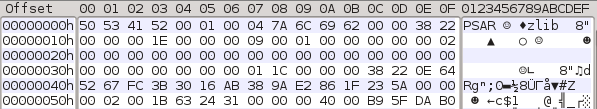
\includegraphics{imgs/CR-PSAR.png}
\caption{Primeros bytes del fichero \texttt{PSAR}.}
\label{fig:met-psar}
\end{figure}

\section{Depuraci�n de c�digo}

% Debate entre ida y no5gba con captura

% TODO: Boku y hebras GZIP

\subsection{B�squeda de archivos en RAM}
% Explicar trauma center

\subsection{B�squeda de algoritmos sobre textos}
\label{sec:met-search-text}
% TODO:
En el Cap�tulo~\ref{sec:translations} se mostrar�n algoritmos para ofuscar y cifrar textos.
El procedimiento para realizar este estudio se basa tanto en depuraci�n de c�digo, como en el conocimiento de malas pr�cticas empleadas.

El primer paso consiste en mirar el archivo cifrado y realizar un estudio de los bytes m�s frecuentes.
Tras una b�squeda de las frases de di�logos iniciales sobre todo el archivo binario del juego no se encuentran resultados.
Se prob� en las codificaciones m�s frecuentes de esta consola como son ASCII y UNICODE sin resultado.
Esto indica que bien el archivo que contiene los textos est� comprimido o cifrado.

El siguiente procedimiento fue extraer la memoria RAM del juego justo en el momento de mostrar ese di�logo, pues deber�a estar almacenada esa frase para poder ser mostrada en pantalla.
Esto se puede realizar gracias al emulador DeSmuME.
Una vez extra�do el archivo binario con la memoria RAM, mediante visores hexadecimales se busc� la frase que aparec�a en pantalla usando las codificaciones est�ndar y sin obtener resultado de nuevo.
Dado que la frase ha de estar en la memoria RAM, el problema era por tanto que no estaba usando una codificaci�n est�ndar.
Existen dos procedimientos b�sicos para realizar una b�squeda en estos casos.

El primero consiste en buscar el archivo con la tipograf�a del juego, pues la codificaci�n ser� la misma que el orden con el que aparecen los caracteres en ella.

El segundo procedimiento posible es el de desarrollar un programa de b�squeda diferencial. Con motivo de este trabajo se explica el programa \textit{RelativeSearch} que se llev� a cabo. Este tipo de software se puede usar siempre y cuando el orden de los caracteres de un mismo grupo (por ejemplo letras min�sculas) corresponda a est�ndares como ASCII. Si se hubiese seguido un orden aleatorio en la codificaci�n propietaria este no servir�a quedando la primera opci�n como �nica alternativa.

Tras usar cualquiera de los dos procedimientos anteriormente descritos, se puedo encontrar una coincidencia en la memoria RAM del di�logo. El siguiente paso consisti� en depurar el juego para hallar el algoritmo de descifrado o descompresi�n de textos. Para ello usando los programas de depuraci�n, se puso un punto de interrupci�n en dicha posici�n.

Cabe destacar que esta posici�n es din�mica por lo que cambia cada vez que se inicia el juego pues depende de muchas variables. Para sortear este problema se hizo uso de los \textit{savestates} del emulador, es decir guardados de memoria del juego que permiten ir a cualquier momento de una ejecuci�n. Gracias a esta caracter�stica se puede realizar un guardado justo antes de que el juego guarde un juego de forma que siempre que se use ese \textit{savestate} encontraremos el texto en la misma posici�n. El punto de interrupci�n hizo parar el emulador justo en las instrucciones m�quinas que estaban realizando, en este caso, el descifrado.

\subsection{B�squeda de algoritmo sobre im�genes}
\label{sec:met-search-img}
El procedimiento para encontrar el algoritmo de cifrado en este caso es distinto al realizado con texto.
No se puede partir de datos conocidos como anteriormente se part�a de una frase que se ve�a en la pantalla.
Sin embargo, dado que las cabeceras de la imagen no est�n cifradas se pudo buscar sobre el c�digo en ensamblador la funci�n que procesa esta cabecera.
En concreto se busc� la palabra m�gica \texttt{CHAR} que se procesa para determinar el comienzo de una secci�n del archivo.

Una vez encontrado la funci�n que lee una imagen, solo habr�a que acceder a una parte del juego donde se esperaba que se cargase una imagen como durante una batalla y poner un punto de interrupci�n sobre esta funci�n.
Tras omitir im�genes que no estaban cifradas\footnote{Dado que una imagen contiene suele tener p�xeles cercanos de igual colores, siempre que en los datos se observara patrones se pod�a determinar que no estaba cifrada.}, se lleg� a una que s� lo estaba donde se puso un punto de interrupci�n.

\section{Intercepci�n de comunicaci�n}
\label{sec:met-nds-desmume}
% explicar desmume modificado para guardar datos

% explicar rc4finder

% explicar sslpatcher

\section{Documentaci�n}

% Explicar databrithm

% Comentar programas de los juegos

% explicar script de organizaci�n

    % Copyright (c) 2015 Benito Palacios S�nchez - All Rights Reserved.
% Esta obra est� licenciada bajo la Licencia Creative Commons Atribuci�n 4.0
% Internacional. Para ver una copia de esta licencia, visita
% http://creativecommons.org/licenses/by/4.0/.

\chapter{Traducciones no oficiales}
\label{sec:translations}
% Traduccion -> parche -> legalidad -> evoluci�n en sagas. Mods. Resultados.

Las traducciones no oficiales, conocidas informalmente como  \textit{fan-traducciones}~\cite{Wiki-Trans}, son trabajos realizados por personas externas a la compa��a desarrolladora.
Su objetivo es traducir un videojuego y compartirlo de forma altruista.
La distribuci�n se hace com�nmente en foros dedicados y mediante \textit{parches}, es decir, archivos binarios que contienen solo las modificaciones realizadas y en principio, no contenido con derechos de autor.
Este cap�tulo se ha centrado en los resultados obtenidos al analizar juegos principalmente de la consola \acl{NDS}.
La selecci�n se ha realizado en base a sagas que han tenenido m�s traducciones no oficiales (\textit{Pok�mon}), juegos con proyectos largos de traducci�n (\textit{Ninokuni}) y aquellos en los que se han visto solicitudes o intentos  (\textit{London Life} y dem�s).

Este tipo de trabajos se remontan al origen de los ordenadores cuando, en 1993 se forma el primer grupo de traducci�n llamado Oasis para MSX~\cite{HarCod-RH}.
A partir de entonces, numeros proyectos han surgido con dos p�ginas webs como referencia: GbaTemp.net\footnote{\url{http://gbatemp.net/}} y ROMHacking.net\footnote{\url{http://www.romhacking.net/}}.
El motivo para iniciar un proyecto es la confirmaci�n por parte de una empresa de que no se llevar�a a cabo la traducci�n del juego.
Como se explica en el �ltimo apartado, a pesar de ello han existido casos en los que la traducci�n se ha iniciado antes de dicha confirmaci�n y tras producirse esta, esos proyectos se detuvieron.
No ha sucedido as� con todos los juegos, pues en la saga de \textit{Pok�mon}, han existido traducciones parciales antes de la oficial, perjudicando las ventas de la compa��a, pues los usuarios prefierer obtener una copia no l�cita del juego antes de esperar a la salida oficial.
Es en estos juegos donde, como se ha analizado en la siguiente secci�n, se observa una evoluci�n de mecanismos para evitar y retrasar estos trabajos.

Estos hechos se han visto reflejados recientemente en dos cartas de \textit{cese y desista} enviadas por la empresa \textit{Square Enix} a los grupos de traducci�n de \textit{Final Fantasy Type-0}~\cite{VG247-FF0} para \ac{PSP} y \textit{Dragon Quest VII}~\cite{Reddit-DQ7} para \acl{N3DS}.
En ellas se alega que por `motivos de mercado' no pueden permitir esos trabajos, refiri�ndose a la salida de estos t�tulos para otras consolas.
En ambos casos, los grupos de traducci�n pararon la traducci�n.

Relacionado con las traducciones, se encuentran los \textit{mods}~\cite{Wiki-Mods}, modificaciones sobre un videojuego con el objetivo de crear una versi�n alternativa.
Usando el motor del juego, se cambia historia, im�genes, sonidos y \textit{scripts}.
Existen comunidades dedicadas exclusivamente a este motivo como es \textit{Whack a Hack!}\footnote{\url{http://wahackpokemon.com/es}} para la saga \textit{Pok�mon}.

Los mecanismos que se van a comentar a continuaci�n, muestran como son los archivos con contenido de texto e im�genes son los m�s protegidos u ofuscados.
Esto no evita en su totalidad la edici�n pues, teniendo acceso al c�digo m�quina que ejecuta la consola, se puede mirar c�mo accede a los ficheros.
Sin embargo, s� puede retrasar o al menos imposibilitar para aquellas personas que no tengan los conocimientos t�cnicos necesarios.

\section{Saga Pok�mon en \acl{NDS}}
\textit{Pok�mon} es una serie de juegos desarrollados por la compa��a \textit{Game Freak} desde el a�o 1993 para las consolas de Nintendo.
Esta saga de juegos se divide en las denominadas `generaciones' que engloban por lo general al menos tres juegos. Sus caracter�sticas es un mismo mapa, con una historia casi id�ntica y un conjunto de \textit{Pok�mon} com�n para conseguir.
Esta ha sido una de las franquicias m�s exitosas a nivel mundial y cuenta con una serie de animaci�n, pel�culas y miles de seguidores.

A causa de su fama, existe siempre un gran n�mero de usuarios que no pueden esperar a que salga en su pa�s para poder jugarlo.
Este es el problema que se deriva de que los juegos se suelan lanzar primero en Jap�n, entorno seis meses m�s tarde en Am�rica y pocos meses despu�s en Europa.
Los usuarios ven que su �nica posibilidad de jugar al juego, a pesar de contar con fechas de localizaci�n confirmadas y exactas, en obtener una copia ileg�tima del juego en un idioma que en la mayor�a de los casos desconocen (japon�s).

Aprovechando esta demanda, en esos meses de intervalos entre fechas de lanzamiento en diversos pa�ses surgen p�ginas webs cuyo objetivo es promocionarse y ganar usuarios lanzando una traducci�n no-oficial y parcial del juego.
Este es el caso de p�ginas que se promocionan con (traducido del ingl�s\footnote{\url{http://pokecheats.net/tools/translations.php}})
\textquote{Pok�Cheats.net est� comenzando a posicionarse en traducciones anticipadas de juegos de Pok�mon de Nintendo que est�n saliendo este a�o. Nuestro objetivo es el de darte una traducci�n de los juegos japoneses en tu idioma, para que puedas comenzar a jugar los pr�ximos t�tulos.}.
En otras ocasiones es gente desinteresada que quiere ayudar a que otras personas disfruten el t�tulo.

En ambos casos, este tipo de traducciones como se coment� en la traducci�n perjudica a la compa��a y es esta la mediante los mecanismos descritos a continuaci�n intenta poner trabas para al menos retrasar estas traducciones y dar tiempo a que salgan las oficiales.

Los textos que aparecen en di�logos y men�s, al igual que aquellos nombres para denominar a \textit{Pok�mons} y ataques son el primer objetivo a la hora de realizar una traducci�n o edici�n.
Es por ello que son estos los archivos m�s protegidos con cifrados u ofuscado de nombre como se ver�.
Cuando mayor sea la protecci�n menos usuarios tendr�n las capacidades y m�s esfuerzo requerir�.
De nuevo se trata el problema descrito en el segundo cap�tulo donde se valora si es el esfuerzo necesario compensa el resultado final.

El �nico tipo de fichero que se ha podido comprobar que en ning�n caso llega a ser protegido son es la m�sica y efectos de sonido del juego, estando en un formato est�ndar con extensi�n \textsf{.sdat} en la carpeta ra�z del juego.

\subsection{Pok�mon Perla y Diamante}
El par de juegos \textit{Pok�mon Diamante y Perla} corresponden a la cuarta generaci�n de saga y a la primera que sali� para \acl{NDS}.
El primer pa�s en recibirlos fue Jap�n a finales de septiembre de 2006 y como es frecuente mucho despu�s lleg� al resto del mundo.
Concretamente pasaron siete meses hasta la llegada a Estados Unidos y tres meses m�s hasta la llegada a Europa.

\subsubsection{Archivos}
Se trata del primera generaci�n de juegos que llegan a esta consola donde como caracter�stica importante respecto a su antecesora (\acl{GBA}) es la introducci�n del sistema de ficheros.
En estos tres juegos, los archivos dentro del juego tienen nombres explicativos sobre su contenido (figura~\ref{fig:tr-pearlfiles}).
Ejemplo son ficheros como \textit{msgdata/msg.narc} con los mensajes o textos del juego, \textit{itemtool/itemdata/item\_icon.narc} con las im�genes de los objetos o \textit{graphic/font.narc} con las tipograf�as del juego.

\includefigure{fig:tr-pearlfiles}%
{Sistema de ficheros en Pok�mon Perla visto con Tinke}%
{imgs/TR-PearlFiles.png}

\subsubsection{Textos}
\label{sec:tr-pok-pearl-text}
Centr�ndose en textos del juego se comprueba que est�n cifrados.
Tras una b�squeda de las frases de di�logos iniciales sobre todo el archivo binario del juego no se encuentran resultados.
Se prob� en las codificaciones m�s frecuentes de esta consola como son ASCII y UNICODE sin resultado.
Esto indica que bien el archivo que contiene los textos est� comprimido o cifrado.

El siguiente procedimiento fue extraer la memoria RAM del juego justo en el momento de mostrar ese di�logo, pues deber�a estar almacenada esa frase para poder ser mostrada en pantalla.
Esto se puede realizar gracias al emulador DeSmuME mencionado en el cap�tulo~\ref{sec:requirements}.
Una vez extra�do el archivo binario con la memoria RAM, mediante visores hexadecimales se busc� la frase que aparec�a en pantalla usando las codificaciones est�ndar y sin obtener resultado de nuevo.
Dado que la frase ha de estar en la memoria RAM, el problema era por tanto que no estaba usando una codificaci�n est�ndar.
Existen dos procedimientos b�sicos para realizar una b�squeda en estos casos.

El primero consiste en buscar el archivo con la tipograf�a del juego, pues la codificaci�n ser� la misma que el orden con el que aparecen los caracteres en ella.
En la tabla~\ref{tab:tr-pearlfont} se especifica el formato usado en este juego para estos archivos.
% TODO: Crear plugin de Tinke para exportarla.
% TODO: A�adir imagen de la tipograf�a extra�da.

\ctable[
    caption = Especificaci�n de tipograf�as en Pok�mon Perla,
    label   = tab:tr-pearlfont,
    pos     = h
]{ccl}{
    \tnote[a]{Los caracteres est�n codificados por \textit{tiles} de 8$\times$x8 p�xeles en formato horizontal.}
    \tnote[b]{Cada byte indica el ancho del car�cter.}
}{                                                                      \FL
    Posici�n      & Tama�o        & Descripci�n                         \ML
    \multicolumn{3}{c}{Cabecera}                                        \NN
    \textsf{0x00} & \textsf{0x04} & Puntero a la secci�n de datos       \NN
    \textsf{0x04} & \textsf{0x04} & Puntero a la secci�n \acs{VWT}      \NN
    \textsf{0x08} & \textsf{0x04} & N�mero de caracteres                \NN
    \textsf{0x0C} & \textsf{0x01} & Ancho de un caracter                \NN
    \textsf{0x0D} & \textsf{0x01} & Alto de un caracter                 \NN
    \textsf{0x0E} & \textsf{0x01} & BPP                                 \NN
    \textsf{0x0F} & \textsf{0x01} & BPP                                 \ML
    \multicolumn{3}{c}{Datos de la fuente\tmark[a]}                     \ML
    \multicolumn{3}{c}{\ac{VWT}\tmark[b]}                               \LL
}

El segundo procedimiento posible es el de desarrollar un programa de b�squeda diferencial. Con motivo de este trabajo en el cap�tulo~\ref{sec:requirements} se explica el programa \textit{RelativeSearch} que se llev� a cabo. Este tipo de \textit{software} se puede usar siempre y cuando el orden de los caracteres de un mismo grupo (por ejemplo letras min�sculas) corresponda a est�ndares como ASCII. Si se hubiese seguido un orden aleatorio en la codificaci�n propietaria este no servir�a quedando la primera opci�n como �nica alternativa.

Tras usar cualquiera de los dos procedimientos anteriormente descritos, se puedo encontrar una coincidencia en la memoria RAM del di�logo. El siguiente paso consisti� en depurar el juego para hallar el algoritmo de descifrado o descompresi�n de textos. Para ello usando los programas descritos en el cap�tulo~\ref{sec:requirements} de depuraci�n, se puso un punto de interrupci�n en dicha posici�n.

Cabe destacar que esta posici�n es din�mica por lo que cambia cada vez que se inicia el juego pues depende de muchas variables. Para sortear este problema se hizo uso de los \textit{savestates} del emulador, es decir guardados de memoria del juego que permiten ir a cualquier momento de una ejecuci�n. Gracias a esta caracter�stica se puede realizar un guardado justo antes de que el juego guarde un juego de forma que siempre que se use ese \textit{savestate} encontraremos el texto en la misma posici�n. El punto de interrupci�n hizo parar el emulador justo en las instrucciones m�quinas que estaban realizando, en este caso, el descifrado. Este algoritmo se describe a continuaci�n.

El texto se encuentra cifrado usando la operaci�n XOR y mediante una clave que se actualiza despu�s de descifrar cada byte\footnote{Al no ser una clave constante no se puede obtener esta al ser aplicada sobre zonas con valores a 0 como s� sucede en el caso de la tabla de contenido.}. La clave inicial es igual a \verb!clave = (ushort)(0x91BD3 * (i + 1))! donde \verb!i! es el bloque de texto a descifrar. Despu�s de aplicar la clave sobre un byte esta se actualiza seg�n \verb!clave = (ushort)(clave + 0x493D)!.

El cifrado no es exclusivo del texto pues la tabla de contenido con las posiciones y tama�os de cada di�logo se encuentra cifrado tambi�n. La clave no coincide con la del texto y se forma de la siguiente manera: \verb!clave = (ushort)(clave_base * 0x2FD * (i + 1))!. En este caso, se hace uso de una clave base que se encuentra disponible en la cabecera del fichero y de nuevo con n�mero de entrada a descifrar (\verb!i!). Dado que el tama�o de estos campos cifrados es de 32 bits y la clave de 16 bits, se concatena la clave dos veces formando el valor de 32 bits necesario para aplicar la operaci�n XOR. % chktex 13

Sin embargo, esta parte del fichero a pesar de estar cifrado presenta un fallo de seguridad. Como se ha comentado los valores cifrados de posici�n y tama�o son de 32 bits (4 bytes) pero en la mayor�a de los casos solo se usan los dos primeros bytes pues tama�o del fichero de texto no supera los \verb!2^16 = 65535 bytes!. Debido a la concatenaci�n de la clave y a que los dos �ltimos bytes son 0, al cifrar estos dos bytes se estuvo guardando la clave en texto plano.
Es decir, se demuestra que \verb!a XOR 0 = a! siendo en este caso \verb!a! la clave para cifrar estas entradas y el valor guardado en el fichero en la mayor�a de los casos.

En la tabla~\ref{tab:tr-pearltxt} se especifica el formato de los archivos de texto.

\ctable[
    mincapwidth = 110 mm,
    footerwidth,
    caption = Especificaci�n del formato de texto en Pok�mon Perla,
    label   = tab:tr-pearltxt,
    pos     = h,
]{ccl}{
    \tnote[a]{Se especifica solo la primera entrada.}
    \tnote[b]{Campo cifrado descrito en la secci�n~\ref{sec:tr-pok-pearl-text}.}
}{                                                                      \FL
    Posici�n      & Tama�o        & Descripci�n                         \ML
    \multicolumn{3}{c}{Cabecera}                                        \NN
    \textsf{0x00} & \textsf{0x02} & N�mero de bloques de texto          \NN
    \textsf{0x02} & \textsf{0x02} & Clave base para descifrar \acs{TIC} \ML
    \multicolumn{3}{c}{\acl{TOC}\tmark[a]}                              \NN
    \textsf{0x00} & \textsf{0x04} & Posici�n del texto\tmark[b]         \NN
    \textsf{0x04} & \textsf{0x08} & Tama�o del texto\tmark[b]           \ML
    \multicolumn{3}{c}{Texto\tmark[b]}                                  \LL
}

\subsubsection{Im�genes}
\label{sec:tr-pok-pearl-img}
En el caso de la saga de Pok�mon las im�genes no contienen frases con texto por lo que en cuanto a una traducci�n respecta no son necesarias editarlas.
Sin embargo, dada la popularidad de los \textit{mods} y de la extracci�n de im�genes en estos juegos se apost� por cifrar un tipo concreto de las mismas.
Se trata de los \textit{sprites} de los \textit{Pok�mons} que aparecen durante las batallas.
Estos archivos est�n contenidos en el paquete \textit{poketool/pokegra/pokegra.narc} donde hay seis im�genes por monstruo.

El cifrado se realiz� sobre los datos de la imagen, manteniendo las cabeceras del formato de la misma sin cifrar.
Como consecuencia, las im�genes se pod�an abrir usando programas est�ndares pero sin ver nada en concreto.
% TODO: Hacer programa y descifrar una imagen y poner comparativa

El procedimiento para encontrar el algoritmo de cifrado en este caso es distinto al realizado con texto.
No se puede partir de datos conocidos como anteriormente se part�a de una frase que se ve�a en la pantalla.
Sin embargo, dado que las cabeceras de la imagen no est�n cifradas se pudo buscar sobre el c�digo en ensamblador la funci�n que procesa esta cabecera.
En concreto se busc� la palabra m�gica \textsf{CHAR} que se procesa para determinar el comienzo de una secci�n del archivo.

Una vez encontrado la funci�n que lee una imagen, solo habr�a que acceder a una parte del juego donde se esperaba que se cargase una imagen como durante una batalla y poner un punto de interrupci�n sobre esta funci�n.
Tras omitir im�genes que no estaban cifradas\footnote{Dado que una imagen contiene suele tener p�xeles cercanos de igual colores, siempre que en los datos se observara patrones se pod�a determinar que no estaba cifrada.}, se lleg� a una que s� lo estaba donde se puso un punto de interrupci�n.

La siguiente funci�n que le�a los datos de dicha imagen era el algoritmo de descifrado. Este algoritmo parte del hecho que todo el bloque de datos de una imagen tendr� el tama�o constante de \textsf{0x1900} bytes.
Se trata de un cifrado parecido al realizado sobre el texto donde habr� una clave que ir� cambiando despu�s de aplicarse sobre cada valor y que se usar� para aplicar la operaci�n XOR sobre un dato cifrado.
En este caso, la clave es de 32 bits y el dato a descifrar de 16 bits y se comencer� desde el final del fichero hasta el principio.
La clave inicial ser� el primer valor (�ltimos dos bytes del fichero) e ir� cambiando siguiendo la siguiente operaci�n \verb!clave = (uint)(clave * 0x41C64E6D + 0x6073)!.

\subsubsection{Conclusi�n}

\begin{tabular}{p{0.4\textwidth}p{0.5\textwidth}}
Puntos fuertes & Puntos d�biles \\
% Pros
\begin{itemize}
\item Los textos usando una codificaci�n no est�ndar.
\item Los textos est�n cifrados con una clave no est�tica.
\item Las im�genes est�n cifradas con un clave no est�tica.
\end{itemize} &

% Contras
\begin{itemize}
\item Los archivos y carpetas tienen nombres descriptivos.
\item Hay un fallo de seguridad en el cifrado de la tabla de contenido de los textos por el que se puede averiguar la clave.
\end{itemize} \\
\end{tabular}

\subsection{Pok�mon HeartGold y SoulSilver}
Los juegos \textit{Pok�mon HeartGold y SoulSilver} son las siguiente generaci�n de la saga que salieron tambi�n para \acl{NDS}.
Se repite como es com�n el orden y plazo de lanzamiento. De esta forma se lanz� primero en Jap�n a mediados de septiembre de 2009, a continuaci�n en Am�rica seis meses despu�s, en abril de 2010, y finalmente en Europa una semana despu�s.

Esta vez no hubo mucha diferencia entre los lanzamientos de Am�rica y Europa lo que provocar�a que no fuese necesario realizar traducciones no oficiales desde el ingl�s, idioma desde el cual al ser m�s sencillo se parten la mayor�a de las traducciones.
Sin embargo, s� hubo traducciones que partieron del japon�s y que se quedaron entorno a un 90\% de finalizaci�n~\cite{PokProj-HG1}.

\subsubsection{Archivos}
\label{sec:tr-pok-heart-file}
La primera gran diferencia en esta generaci�n llega con el ofuscado de nombres de archivos y directorios. Como se puede apreciar en la figura~\ref{fig:tr-heartfiles} todos los archivos principales del juego est�n nombrados con n�meros y clasificados en carpetas num�ricas tambi�n.
Adem�s, el contenido de estas carpetas no relaciona a los archivos entre s� generando una organizaci�n aleatoria.
En total hay 275 archivos que a su vez son contenedores de subarchivos sin nombre.
Estos contenedores pueden llegar a tener m�s de 1000 archivos en su interior pero si se garantiza que el contenido de estos est� relacionado entre si correspondiendo a las im�genes a las caracter�sticas de \textit{Pok�mon} o las im�genes de un men� concreto.

\includefigure{fig:tr-heartfiles}%
{Carpetas y ficheros ofuscados en Pok�mon HeartGold}%
{imgs/TR-HeartFiles.png}

Mediante depuraci�n del c�digo ensamblador se pudo comprobar la implementaci�n del acceso a estos archivos.
Todo se realiza llamando a varias funciones de similar cometido cuyo primer par�metro es un ID que identifica al archivo y como segundo par�metro el sub-archivos dentro del contenedor.
Este ID es lineal y si se descompone en base diez se puede calcular la ruta absoluta.
De esta forma el ID \textsf{0x1B} (27) corresponde a \verb!27 = 0*10 + 2*10 + 7! lo que significa que estar�a ubicado en \textit{a/0/2/7}.
A la hora de implementar este mecanismo durante el desarrollo del videojuego se usuar�a un archivo de cabeceras similar al siguiente.

\begin{verbatim}
file_paths.h
#define MESSAGE_FILE_ID 0x1B
#define POKEMON_IMAGES_FILE_ID 0x1C
\end{verbatim}

De esta manera, en el proceso de desarrollo ser�a f�cil y sin ofuscar su propio c�digo el indicar qu� fichero cargar usando las constantes definidas.
Este m�todo es sencillo de implementar y dificulta la tarea de edici�n del juego pues entre los 275 archivos disponibles, binarios, sin estructuras de datos conocidas, habr�a que averiguar qu� hace cada uno sin tener una pista previa como pasaba en ediciones anteriores donde el nombre era descriptivo del contenido.

\subsubsection{Textos}
Los textos de esta generaci�n vienen igualmente cifrados.
Esto se pudo comprobar al realizar de nuevo una b�squeda de palabras de los primeros di�logos y no tener resultados ni en el archivo binario del juego ni sobre la memoria RAM.

Tras repetir el proceso descrito en la secci�n~\ref{sec:tr-pok-pearl-text} de textos de la generaci�n anterior, se comprob� que tanto el formato del archivo como el algoritmo de cifrado y claves son exactamente las mismas a las descritas ah�. Adem�s el formato de las fuentes es tambi�n el mismo.

En esta nueva generaci�n no se apost� por cambiar el cifrado de textos y delegar toda la responsabilidad de dificultar la tarea de edici�n en el ofuscamiento de nombres de ficheros. El fichero est� localizado en \textit{a/0/2/7}.

\subsubsection{Im�genes}
Al igual que sucede con los textos, tras repetir los pasos de la secci�n~\ref{sec:tr-pok-pearl-img} de im�genes se descubri� que se utiliza el mismo algoritmo de cifrado con las mismas claves. Se encontr� sin embargo, una diferencia en la implementaci�n pues en este caso se descifra empezando por el comienzo de los datos en lugar de por el final.

\subsubsection{Conclusi�n}

\begin{tabular}{p{0.4\textwidth}p{0.5\textwidth}}
Puntos fuertes & Puntos d�biles \\
% Pros
\begin{itemize}
\item Los archivos est�n ofuscados por nombre y directorio.
\end{itemize} &

% Contras
\begin{itemize}
\item No todos los archivos est�n ofuscados como se ve en la siguiente apartado.
\item Se mantiene los mismos algoritmos y claves que en la generaci�n anterior por lo que una vez encontrado los archivos se pueden reutilizar las mismas herramientas.
\end{itemize} \\
\end{tabular}

\subsection{Pok�mon Blanco y Negro}
La sexta generaci�n corresponde a los juegos \textit{Pok�mon Blanco y Negro} para la \acl{NDS}.
Primero salieron en Jap�n a mediados de septiembre de 2010 y a principios de marzo de 2011 en Am�rica y Europa.
Esta vez, como curiosidad, el juego sali� por primera vez dos d�as antes en Europa que en el resto de sitios.

De nuevo esta edici�n fue esperada por muchos seguidores que unido con el avance que hay en el mundo de la ingenier�a inversa para la \acl{NDS} en estos a�os, facilit� la tarea de traducci�n no oficial~\cite{PokProj-BW1}.
No solo llegaron a salir traducciones al ingl�s si no tambi�n a otros idiomas como espa�ol.
Todas ellas se llevaron a cabo de forma transparente y colaborativa mediante GitHub\footnote{\url{https://github.com/projectpokemon/Pokemon-Black-White-Translation-Files}}.

\subsubsection{Archivos}
En la sexta generaci�n decidieron optar de nuevo por ofuscar los nombres de las carpetas y archivos.
En este caso, se dio un paso m�s y se hizo sobre todos los archivos.
Sin bien, en el caso de \textit{Pok�mon HeartGold y SoulSilver} fueron solo los archivos principales los ofuscados, en esta edici�n los �nicos que no se procesaron fueron los de sonido y demo como se aprecia en la figura~\ref{fig:tr-blackheartfiles}.

\includefigure{fig:tr-blackheartfiles}%
{Comparaci�n de carpetas entre Pok�mon Blanco (izq.) y Pok�mon HeartGold (der.)}
{imgs/TR-BlackHeartFiles.png}

A pesar de usar internamente la misma forma de acceso a como se describi� en el apartado de archivos de la secci�n~\ref{sec:tr-pok-heart-file}, los identificadores y por tanto localizaci�n de estos cambi�.
Pasando de esta forma el archivo con los textos del juego a estar en \textit{a/0/0/2} en lugar de \textit{a/0/2/7} como suced�a en la edici�n anterior.

\subsubsection{Textos}
\label{sec:tr-pok-black-text}
En el apartado de protecci�n a los textos, en las dos generaciones anteriores se utiliz� un mismo algoritmo basado en un clave din�mica que se aplicaba con la operaci�n XOR. En esta generaci�n la filosof�a del algoritmo se mantiene cambiando no obstante la forma de generaci�n y actualizaci�n de la clave.
Esta se pudo obtener tras realizar el procedimiento descrito en el apartado textos de la secci�n~\ref{sec:tr-pok-pearl-text}.

La principal diferencia tras aplicar el m�todo de investigaci�n de cifrado fue ver que no se usaba una codificaci�n propia si no UTF-16.
Esto facilit� la tarea, pues ya no es necesaria una b�squeda diferencial en la memoria RAM y por tanto crear \textit{software} adicional para investigar.
Se trata por tanto de la eliminaci�n de un mecanismo fuerte a la hora de proteger datos que posiblemente estaba realizando en ediciones anteriores de casualidad.

La clave inicial usada para el texto se genera usando el n�mero de bloque como variable, de forma que cada bloque comienza con una clave diferente. La operaci�n es \verb!clave = (i + 3) * 0x2983!.
Tras aplicar esta clave sobre un valor de 16 bits cifrado (dos bytes), se actualiza desplazando los tres bits m�s significados a la posici�n menos significativa.
Esto se puede conseguir aplicando la siguiente serie de operaciones.

\begin{verbatim}
temp  = clave & 0x1FFF;             // Elimina los bits m�s significativos
clave = (temp << 3) | (clave >> 13) // y los a�ade al principio.
\end{verbatim}

Al desplazarse un n�mero impar de veces, cada bit pasar� de forma lineal sobre cada posici�n de la clave obteni�ndose el m�ximo de permutaciones para una clave de 16 bits, es decir se usar� a la hora de cifrar y descifrar 16 claves diferentes.

La estructura de datos se especifica en la tabla~\ref{tab:tr-blacktxt} donde se puede ver que la secci�n con la tabla de contenido no est� cifrada a diferencia de c�mo pasaba en ediciones anteriores.

\ctable[
    mincapwidth = 110 mm,
    footerwidth,
    caption = Especificaci�n del formato de texto en Pok�mon Blanco,
    label   = tab:tr-blacktxt,
    pos     = h,
]{ccl}{
    \tnote[a]{Se especifica solo la primera entrada.}
    \tnote[b]{Cada car�cter es un valor de 16 bits.}
    \tnote[c]{Campo cifrado descrito en la secci�n~\ref{sec:tr-pok-black-text}.}
}{                                                                          \FL
    Posici�n      & Tama�o        & Descripci�n                             \ML
    \multicolumn{3}{c}{Cabecera}                                            \NN
    \textsf{0x00} & \textsf{0x02} & Constante: \textsf{0x01}                \NN
    \textsf{0x02} & \textsf{0x02} & N�mero de bloques de texto              \NN
    \textsf{0x04} & \textsf{0x04} & Tama�o de la secci�n de datos           \NN
    \textsf{0x08} & \textsf{0x04} & Constante: \textsf{0x00}                \NN
    \textsf{0x0C} & \textsf{0x04} & Tama�o de la cabecera                   \ML
    \multicolumn{3}{c}{Datos}                                         \NN
    \textsf{0x00} & \textsf{0x04} & Tama�o de la secci�n                    \NN
    \textsf{0x04} & \textsf{0x04} & Posici�n relativa a la secci�n\tmark[a] \NN
    \textsf{0x06} & \textsf{0x02} & N�mero de caracteres\tmark[a]\tmark[b]  \NN
    \textsf{0x08} & \textsf{0x02} & Desconocido\tmark[a]                    \ML
    \multicolumn{3}{c}{Texto\tmark[c]}                                      \LL
}

\subsubsection{Im�genes}
Las im�genes a diferencia de las pasadas generaciones no se cifraron.
En cambio, no se utiliza un formato est�ndar de codificaci�n.
Si bien el formato para las paletas y datos de imagen si se reutiliza y sigue siendo est�ndar, existe un ficheros extras con una especificaci�n nueva en este juego con la informaci�n necesaria para recomponer la imagen (figura~\ref{fig:tr-blackimg}).

\includefigure{fig:tr-blackimg}%
{Im�genes sin cifrar en Pok�mon Negro.}%
{imgs/TR-BlackImg.png}

Esta forma de codificaci�n, aunque pudiendo no ser espec�fica para protegerlas ante modificaciones si no un requisito para animaciones, es m�s fuerte.
De esta forma los programas de ediciones gen�ricas creados para juegos de \acl{NDS} ya no son �tiles y se necesita nuevos y espec�ficos.
Esta tarea requiere de investigaci�n de formatos y de programaci�n, algo que toma m�s esfuerzo y tiempo que crear un decodificador como pasaba en las generaciones anteriores.

A pesar de ello, esta reconstrucci�n y edici�n de la imagen se podr�a llegar a cabo manualmente ya que el formato de los ficheros principales: paleta y datos de imagen, sigue siendo el est�ndar para juegos de la \acl{NDS}.

\subsubsection{Conclusi�n}

\begin{tabular}{p{0.4\textwidth}p{0.5\textwidth}}
Puntos fuertes & Puntos d�biles \\
% Pros
\begin{itemize}
\item Los nombres de las carpetas y archivos est�n ofuscados.
\item Los textos est�n cifrados con un nuevo algoritmo y clave.
\item Las im�genes usan archivos extras con especificaciones nuevas para recomponerlas por lo que \textit{software} nuevo ser�a necesario.
\end{itemize} &

% Contras
\begin{itemize}
\item Los textos no usan una codificaci�n propia.
\item Las im�genes no est� cifradas.
\item Las im�genes usando el formato est�ndar para los archivos principales.
\end{itemize} \\
\end{tabular}

\subsection{Pok�mon Conquest}
\textit{Pok�mon Conquest} es un juego desarrollado por \textit{Tecmo Koei} y publicado en el a�o 2012 para la consola \acl{NDS}.
Este juego dista de la mec�nica de la saga principal pues se trata de un g�nero de combates por turnos y estrategia en lugar de RPG. Primero se distribuy� en Jap�n a mediados de marzo, y a pesar de que tardaron meses en confirmarlo, en junio y julio del mismo a�o se lanz� en Am�rica y Europa.

Esta falta de confirmaci�n inicial hicieron incluso tres d�as antes del lanzamiento se formara un grupo de traducci�n no oficial con el objetivo de ofrecer una jugabilidad parcial lo m�s pronto posible~\cite{PokCheat-Conq}.
Esta traducci�n lleg� a casi completarse al ingl�s en cuanto a la trama principal y listas de nombres.
Adem�s surgieron a partir de esta varias a otros idiomas como italiano y alem�n.

\subsubsection{Archivos}
En este juego no se han ofuscado los archivos y carpetas.
Todo est� bien organizado y con nombres descriptivos.

\subsubsection{Textos}
\label{sec:tr-pok-conquest-text}
Los textos s� han cifrado y codificado con una protecci�n mayor que en otras generaciones.
Para encontrar se busc� en primer lugar sobre la memoria RAM repitiendo el proceso explicado en el apartado textos de la secci�n~\ref{sec:tr-pok-pearl-text}.
Dado que se usa la codificaci�n est�ndar SJIS se pudo encontrar directamente.

Una vez puesto el punto de interrupci�n se dio con el algoritmo que descodifica estos caracteres.
Con el objetivo de ahorra espacio y ofuscar el texto los archivos de textos tienen una codificaci�n especial basada en caracteres de control y optimizada para caracteres japoneses.
Su sistema se basa en especificar solo un byte por car�cter japon�s en lugar de dos como dice SJIS.
El segundo car�cter restante al estar comprendido entre \textsf{0x81--0x83} y es igual entre caracteres cercanos, se va predice mediante unos c�digos de control.
Esta codificaci�n est� implementada en ambos sentidos en el proyecto AmbitionText\footnote{\url{http://subirelcodigo}}.
Destaca esta codificaci�n pues no es sencilla de implementar y requiere mucho esfuerzo de creaci�n de una herramienta que permita trabajar con ella.

Antes de esta parte de codificaci�n, el texto se descifra.
El cifrado se basa en aplicar la clave ``\textsf{MsgLinker Ver1.00}'' sobre cada byte de texto.
A continuaci�n se muestra la implementaci�n en C\# para el cifrado y descifrado\footnote{\url{http://subirelcodigo}}.
El formato del fichero se especifica en la tabla~\ref{tab:tr-conquesttxt}.

\begin{verbatim}
string key = "MsgLinker Ver1.00";
for (int i = 0; i < data.Length; i++)
    data[i] ^= key[i % key.Length];
\end{verbatim}

\ctable[
    caption = Especificaci�n del formato de texto en Pok�mon Conquest,
    label   = tab:tr-conquesttxt,
    pos     = h,
]{ccl}{
    \tnote[a]{Se especifica solo la primera entrada.}
    \tnote[b]{Existen 33 bloques.}
    \tnote[c]{Campo cifrado descrito en la secci�n~\ref{sec:tr-pok-conquest-text}.}
}{                                                                          \FL
    Posici�n      & Tama�o        & Descripci�n                             \ML
    \multicolumn{3}{c}{\acl{TOC}\tmark[a]\tmark[b]}                         \NN
    \textsf{0x00} & \textsf{0x04} & Posici�n del bloque                     \NN
    \textsf{0x04} & \textsf{0x04} & Tama�o del bloque                       \ML
    \multicolumn{3}{c}{Bloques\tmark[c]}                                    \LL
}

\subsubsection{Im�genes}
Tanto los fondos como los \textit{sprites} del juego no vienen cifrados.
Sin embargo se usan formatos de ficheros nuevos, con codificaciones nuevas que supusieron un trabajo extra de creaci�n de \textit{software}\footnote{\url{https://github.com/pleonex/tinke/tree/master/Plugins/PSL}}.

\subsubsection{Conclusi�n}

\begin{tabular}{p{0.4\textwidth}p{0.5\textwidth}}
Puntos fuertes & Puntos d�biles \\
% Pros
\begin{itemize}
    \item Los textos vienen cifrados y codificados.
    \item La codificaci�n es �nica para este juego.
    \item Nuevos formatos de im�genes que requieren nuevos programas.
\end{itemize} &

% Contras
\begin{itemize}
    \item Los archivos y carpetas no est�n ofuscados.
    \item Se usa una codificaci�n final est�ndar.
    \item Las im�genes no est�n cifradas.
\end{itemize} \\
\end{tabular}

\section{Ninokuni y el Mago de las Tinieblas}
\textit{Ni no Kuni: Shikkoku no Madoshi} es el t�tulo original de un juego que solo lleg� a Jap�n de la mano de \textit{Level-5} para la consola \acl{NDS} en 2010.
Desde su salida, debido a que el juego se distribu�a junto a un libro f�sico, se confirm� que iba a poder salir de este pa�s debido a los costes de producci�n y traducci�n que supondr�a el libro.

Es por ello, que a finales de 2011 un grupo denominado GradienWords\footnote{\url{http://gradienwords.com}} se form� con el objetivo de realizar una traducci�n altruista del juego.
Este proyecto termin� a finales de mayo de 2015 e incluye tanto el juego como una copia del libro en PDF traducida.
Con fecha de este trabajo este es el �nico proyecto de traducci�n de este juego que se ha finalizado, a pesar de que est�n en marcha varios al franc�s, ingl�s e italiano\footnote{\url{http://gbatemp.net/forums/nds-rom-hacking-and-translations.41/}}.

El juego se lleg� a lanzar previamente en \acl{PS3} en varios idiomas incluyendo el espa�ol pero no lleg� con la copia f�sica del libro y tanto la mec�nica del juego como la historia se cambiaron.

La protecci�n encontrada en este juego muestra no se concentra en evitar una traducci�n, posiblemente porque la compa��a sab�a que ellos no lo iban a hacer, si no modificaciones del juego.
De esta forma se aprecia como los archivos que contienen par�metros como caracter�sticas de los monstruos, de ataque y batalla s� est�n cifrados.
Adem�s de como se explicar� el archivo de guardado tambi�n presenta un algoritmo de integridad.

\subsubsection{Archivos}
Los archivos y carpetas no est�n ofuscadas y est� todo bien organizado y clasificado.

\subsubsection{Textos}
En cuanto al apartado de textos hay que distinguir de dos tipos: \textit{scripts} y nombres y descripciones.
Empezando por el �ltimo, este tipo de textos se encuentran en archivos que contienen las caracter�sticas de personajes, objetos y ataques y no solo el texto.
Con el objetivo de editar los par�metros que definen sus caracter�sticas y hacer una versi�n modificada del mismo con mayor, menor o una jugabilidad distinta estos ficheros se cifraron.
El cifrado es muy b�sico y pero eficaz ante personas que no entienden.
En la figura~\ref{fig:tr-nino-minitext} se puede ver como se repite el byte \textsf{0xFF} con frecuencia.
Esto da una pista del tipo de cifrado empleado pues probando a realizar una operaci�n \textsf{XOR 0xFF} o lo que es lo mismo \textsf{NOT} se puede ver como todo queda descifrado.

\includefigure{fig:tr-nino-minitext}%
{Archivo cifrado (arr.) y descifrado (ab.) de Ninokuni y el Mago de las Tinieblas}%
{imgs/TR-NinoMiniText.png}

Respecto a los \textit{scripts} debido a sus requisitos t�cnicos para ejecutar todo tipo de comandos son complejos de investigar.
A d�a de hoy solo existe un \textit{software} no p�blico desarrollado para la traducci�n al espa�ol que solo es capaz de editar los textos de los di�logos.
El formato est� basado en par�metros a nivel de bits lo que hace inviable investigar el formato sin mirar las instrucciones m�quinas del juego que lo procesan.

\subsubsection{Im�genes}
Las im�genes no est�n cifradas pero los archivos asociados a una imagen est�n comprimidos en un nuevo formato.
Son f�ciles de extraer pero requiere nuevo \textit{software}\footnote{\url{https://github.com/pleonex/ninoimager}}.

\subsubsection{Integridad en archivos de guardado}
En este videojuego se ha estudiado adicionalmente los mecanismos de protecci�n en el archivo con los datos de guardado.
Se trata de un fichero que en los cartuchos originales no se puede editar sin poseer \textit{hardware} adicional pero que en una \textit{flashcard} se trata de un fichero com�n, en este caso de 64 KB, y que por tanto es accesible y f�cil de editar de forma no autorizada.

Para evitar esto mismo, en lugar de cifrar se ha apostado por implementar un algoritmo de integridad.
Para encontrarlo se busc� en la memoria RAM extra�da con el emulador DeSmuME, los datos de este archivo.
Una vez localizada la parte de la memoria que contiene el archivo, se puso un punto de interrupci�n en los primeros bytes para conocer qu� operaciones se realizan sobre los mismos.

En primer lugar se comprueba que el primer valor de 16 bits sea \textsf{0x0028} y que los �ltimos ocho bytes sean en hexadecimal \textsf{0B 3F A5 84 EC 32 9A 7D}.
A continuaci�n sobre el resto de los datos, desde la posici�n \textsf{0x0002} hasta \textsf{0xFFE4} se calcula un hash usando el algoritmo SHA-1.
Para a�adir seguridad e imposibilitar la edici�n sin conocer todos los detalles de la implementaci�n, lo requiere mirar estas instrucciones m�quinas, en la posici�n \textsf{0xC5EC} durante el c�lculo del hash se escriben los bytes en hexadecimal \textsf{6E 6B 6E 6E} (en ASCII y \textit{low-endian} equivalen a las consonantes del nombre del juego `\textit{nnkn}').
Se trata de una clave que sin conocer ni su valor ni su posici�n ser�a imposible calcular un c�digo SHA-1 v�lido.
Este hash se guarda en la posici�n \textsf{0xFFE4} del archivo de guardado y durante el inicio del juego se comprueba.
En caso de no ser v�lido el mensaje muestra un mensaje de error y borra todos los datos de la partida.

\includefigure{fig:tr-ninosaveinvalid}%
{Mensaje de error al detectar una partida modificada (izq.) y advertencia (der.).}%
{imgs/TR-NinoSaveInvalid.png}

\subsubsection{Conclusi�n}

\begin{tabular}{p{0.4\textwidth}p{0.5\textwidth}}
Puntos fuertes & Puntos d�biles \\
% Pros
\begin{itemize}
    \item Formato complejo en los \textit{scripts}.
    \item Cifrado b�sico en algunos archivos de texto.
    \item Mecanismo de integridad en el archivo de guardado.
\end{itemize} &

% Contras
\begin{itemize}
    \item En general los archivos no est�n cifrados los archivos de texto.
    \item Las im�genes no est�n cifradas.
\end{itemize} \\
\end{tabular}

\section{Proyectos abandonados}
Para terminar se incluye un estudio sobre los proyectos de traducciones no oficiales que han sido abandonados con fecha de este trabajo y con sus respectivos motivos.
El estudio se ha centrado en juegos para la \acl{NDS} a partir de~\cite{GTemp-Aband} y~\cite{RH-Aband}.

El objetivo ser� el de mostrar las causas m�s frecuentes que como se ver� en la mayor�a de los casos fue por la confirmaci�n de una localizaci�n al idioma de la traducci�n.

\subsubsection{Ausencia de \textit{software} de edici�n}
Surgidos por la falta de personal con conocimientos t�cnicos y de programaci�n que puedan crear los programas necesarios de edici�n.
\begin{itemize}
\item WWII-Tank Battles (\acs{PS2}): Ausencia de descompresor de archivos.
\item Chi's Sweet Home: Chi ga Ouchi ni Yatte Kita! (\acs{NDS}): Ausencia de importador de im�genes.
\item Brave Fencer Musashi (\acs{PSX}): Ausencia de editor de textos.
\item Code Geass: Hangyaku no Lelouch (\acs{NDS}): Ausencia de editor de textos.
\item Custom Beat Battle Draglade 2 (\acs{NDS}): Ausencia de editor de textos.
\item Mobile Suit Gundam 00 (\acs{NDS}): Ausencia de editor de textos.
\item Super Robot Taisen OG Saga: Mugen No Frontier (\acs{NDS}): Ausencia de editor de textos.
\item Mysterious Dungeon: Shiren the Wanderer 2 (\acs{NDS}): Ausencia de editor de textos y de modificaciones t�cnicas necesarias sobre el juego.
\end{itemize}

\subsubsection{Problemas t�cnicos tras editar el juego}
Problemas surgidos durante la traducci�n que no se solucionaron debido a falta de conocimientos o abandono de soporte de quienes crearon las herramientas.
\begin{itemize}
\item Dai Kaijuu Monogatari (\acs{PSX}): Los programas usados para editar los textos causan bloqueos en el juego.
\item Resident Evil 2 (\acs{DC} y \acs{GC}): El compresor de archivos creado no funcionaba con todos.
\end{itemize}

\subsubsection{Abandono personal}
Causado en su mayor�a por una falta de motivaci�n y tiempo del equipo que lo llevaba a cabo.
\begin{itemize}
\item Professor Layton: London Life (\acs{NDS}).
\item Cross Treasures (\acs{NDS}).
\item Element Hunters (\acs{NDS}).
\item Hajime no Ippo The Fighting! DS (\acs{NDS}).
\item Naruto: Ninja Destiny 3 (\acs{NDS}).
\item Super Robot Wars K (\acs{NDS}).
\end{itemize}

\subsubsection{Traducci�n oficial}
Abandonos de proyectos por la llegada o confirmaci�n de una traducci�n oficial.
\begin{itemize}
\item Final Fantasy: The 4 Warriors of Light (\acs{NDS}). Traducci�n inglesa.
\item Fire Emblem: Shadow Dragon (\acs{NDS}).
\item Glory of Heracles (\acs{NDS}).
\item Inazuma Eleven (\acs{NDS}).
\item Kindom Hearts 356/2 Days (\acs{NDS}).
\item Naruto: Ninja Destiny 2 (\acs{NDS}).
\item Nostalgia (\acs{NDS}).
\end{itemize}

Se puede ver que el problema m�s com�n est� la falta de programas de edici�n de juegos concretos.
Para poder llevar a cabo esto hace falta unos conocimientos t�cnicos tanto de \textit{software} como de \textit{hardware} y de una larga experiencia.
Es por esto que a la hora de empezar un proyecto la parte t�cnica suele ser la m�s complicada de resolver y que en muchos casos nunca se llega a resolver del todo.

La segunda causa m�s frecuente es la confirmaci�n de la llegada de una localizaci�n, suficiente motivo para parar el proyecto y no da�ar los intereses de mercado de una empresa.

    % Copyright (c) 2015 Benito Palacios S�nchez - All Rights Reserved.
% Esta obra est� licenciada bajo la Licencia Creative Commons Atribuci�n 4.0
% Internacional. Para ver una copia de esta licencia, visita
% http://creativecommons.org/licenses/by/4.0/.

\chapter{Contenido con derechos de autor}
\label{sec:copyright}
% DRM -> Tipos DRM -> Agujero anal�gico -> Mi an�lisis.
La gesti�n de los derechos de autor ha generado un debate, que sigue sin estar resuelto, entre la libertad del usuario y la protecci�n del creador de la obra~\cite{EurAct-CPR}.
Este incluye a los videojuegos, donde la pirater�a causa p�rdidas millonarias~\cite{DRM-Game-Carolina}.
De este contexto nace la idea del \ac{DRM}, un mecanismo para imposibilitar la distribuci�n no autorizada de contenidos.

Las caracter�sticas de estas t�cnicas se resumen en: detectar qui�n accede a cada obra, cu�ndo y bajo qu� condiciones, autorizar o denegar de manera inapelable el acceso y autorizarlo bajo condiciones restrictivas~\cite{Wiki-DRM}.
En cuanto a mecanismos que se aplican para evitar la distribuci�n ileg�tima, los m�s comunes son~\cite{DRM-Game-Carolina}:

\begin{itemize}
\item Claves en CD.
Se imprim�a en la superficie del CD una clave que se ped�a durante la instalaci�n.
La parte negativa es que si se perd�a esta clave, el usuario leg�timo no pod�a acceder, adem�s del hecho de que con una simple b�squeda en Internet se pod�a obtener.

\item L�mite de instalaciones.
Uno de los siguientes m�todos fue controlar el n�mero de instalaciones.
Para ello, el producto se ten�a que activar realizando una conexi�n con los servidores de la compa��a.
Sin embargo, esto requiere que el usuario tenga acceso a Internet y  que los servidores est�n activos.
Adem�s, limita el n�mero de dispositivos del usuario.

\item Conexi�n permanente (\textit{Always-on DRM}~\cite{Wiki-AlwaysOn}).
Este m�todo necesita una conexi�n en cada inicio del juego con los servidores de la compa��a, e incluso en algunos casos durante toda la partida.
Esto ha causado pol�mica debido a que el usuario no podr�a jugar sin conexi�n a Internet y porque los servidores tienen que estar activos todo el tiempo\footnote{Algunos juegos de la compa��a \textit{Ubisoft} se quedaron sin acceso por tiempo indefinido debido a tareas de mantenimiento de los servidores: \url{http://www.gamespot.com/articles/ubisoft-drm-games-to-be-temporarily-unplayable/1100-6349732/}}.

\item Cifrado del software.
Consiste en cifrar la aplicaci�n usando claves asim�tricas~\cite{iOS-Encryption}.
Como contrapartida, si el usuario pierde su clave privada y el acceso a ella, no podr�a volver a ejecutar ninguna aplicaci�n.
\end{itemize}

El principal problema es la posibilidad de aplicar m�todos de \textit{ingenier�a inversa} sobre el software autorizado.
Una vez comprendido c�mo una aplicaci�n autorizada accede al contenido protegido, se podr�an superar los mecanismos de protecci�n para extraer, y en algunos casos modificar, el recurso.
De aqu� viene la necesidad de trabajar sobre entornos cerrados (Cap�tulo~\ref{sec:art}) cada vez m�s frecuentes en videoconsolas y m�viles\footnote{Los sistemas operativos iOS y Android no permiten el acceso al sistema de ficheros por defecto.}.
Una alternativa ser�a implementar el algoritmo en hardware como es el caso de la \acl{N3DS}.

A�n encontrando un algoritmo eficiente en t�rminos de protecci�n y sin sobrecarga a la hora de procesado, una vulnerabilidad inevitable es el denominado \textbf{\textit{agujero anal�gico}}.
La t�cnica consiste en reconvertir un medio digital en anal�gico, perdiendo los mecanismos DRM.
Por ejemplo, grabar m�sica que se est� reproduciendo con un micr�fono, grabar con una c�mara una pantalla, escanear un libro o incluso copiarlo a mano.
Estos procedimientos se utilizan en los videojuegos para, mediante funciones del emulador como capturas de pantalla o grabaci�n de audio, extraer y compartir recursos en p�ginas como \textit{Spriters Resource}\footnote{\url{http://www.spriters-resource.com/}}.

En las siguientes secciones se analizar�n los posibles mecanismos de seguridad que los juegos aplicar�an sobre contenidos con derechos de autor.
Para ello se han escogido una serie de juegos conocidos por tener materiales que frecuentemente son protegidos~\cite{SurveyDrm}.
En primer lugar se analizar�n juegos con libros electr�nicos, a continuaci�n se investigar� el g�nero \textit{m�sical} y la protecci�n sobre el material filmogr�fico.
El resultado en todos los casos ha sido la carencia de cualquier mecanismo a la hora de proteger los contenidos, exceptuando en el material en formato de v�deo descrito en la �ltima secci�n.
Tambi�n destaca la distribuci�n de material adicional como el caso de un libro f�sico en \textit{Ninokuni} para \acl{NDS} o hardware en la saga \textit{Guitar Hero: On Tour}.

\section{Libros electr�nicos}
\label{sec:cr-ebook}
\subsection{Ninokuni: La Ira de la Bruja Blanca}
\label{sec:cr-nino}
\textit{Ninokuni: La Ira de la Bruja Blanca} es un juego desarrollado por \textit{Level-5} para \acl{PS3} en el a�o 2011.
En el Cap�tulo de traducciones no oficiales (\ref{sec:tr-nino}) se expusieron los resultado del an�lisis de este juego para \acl{NDS}.
En esa versi�n se inclu�a un libro f�sico necesario durante el desarrollo del juego.
Sin embargo, en \acl{PS3} se incluye digitalmente y se puede acceder a �l mediante un visor integrado en el juego.

El libro se encuentra en el archivo \texttt{hd05\_es.sdat}, dentro de la carpeta ra�z y en formato \texttt{PSAR}.
Este tipo de formato, com�n en juegos de \acs{PS3}, permite agrupar varios archivos y comprimirlos.
La compresi�n, \texttt{zlib}, se indica claramente con cuatro caracteres en la posici�n \texttt{0x08} (Figura~\ref{fig:met-psar}).
Respecto a la estructura del fichero (Tabla~\ref{tab:cr-psar}), tiene una peque�a cabecera a la que le sigue una tabla de contenidos y los datos.
En GitHub hay repositorios con programas para la extracci�n de los archivos\footnote{\url{https://github.com/pleonex/Ninokuni/tree/master/Programs/PS3/NinoDecompiler}}.

\ctable[
    caption = Especificaci�n de formato \texttt{PSAR}.,
    label   = tab:cr-psar,
    pos     = tb
]{ccl}{
    \tnote[a] {Los archivos pueden estar comprimidos.}
    \tnote[b] {El primer archivo con c�digo MD5 nulo contiene la lista de nombres y rutas de ficheros.}
}{                                                                      \FL
    Posici�n      & Tama�o        & Descripci�n                         \ML
    \multicolumn{3}{c}{Cabecera}                                        \NN
    \texttt{0x00} & \texttt{0x04} & Identificador: \texttt{PSAR}        \NN
    \texttt{0x04} & \texttt{0x04} & Versi�n: \texttt{0x00010004}        \NN
    \texttt{0x08} & \texttt{0x04} & Compresi�n: \texttt{zlib}           \NN
    \texttt{0x0C} & \texttt{0x04} & Posici�n de los datos               \NN
    \texttt{0x10} & \texttt{0x04} & Tama�o de la siguiente secci�n      \NN
    \texttt{0x14} & \texttt{0x04} & N�mero de archivos                  \NN
    \texttt{0x18} & \texttt{0x04} & Reservado                           \NN
    \texttt{0x1C} & \texttt{0x04} & Reservado                           \ML
    \multicolumn{3}{c}{\textit{File Info Table}}                        \NN
    \texttt{0x00} & \texttt{0x10} & C�digo MD5 del nombre del fichero   \NN
    \texttt{0x10} & \texttt{0x04} & Desconocido                         \NN
    \texttt{0x14} & \texttt{0x05} & Posici�n de los datos               \NN
    \texttt{0x19} & \texttt{0x05} & Tama�o de los datos                 \ML
    \multicolumn{3}{c}{Archivos\tmark[a]\tmark[b]}                      \LL
}

Descomprimiendo el fichero se encuentran nueve archivos, de los cuales destaca uno de 438 MB en \texttt{data/book/es/BigData/gdv.dat} donde se encuentra el libro.
El formato se especifica en la Tabla~\ref{tab:cr-gvd}.
Destaca que la codificaci�n de las p�ginas viene especificada de forma visible con los caracteres \texttt{JPEG} en una de las cabeceras.

\ctable[
    caption = Especificaci�n de formato \texttt{GVD}.,
    label   = tab:cr-gvd,
    pos     = tb
]{ccl}{
    \tnote[a]{Hay un bloque por p�gina.}
    \tnote[b]{Relativo al inicio del bloque de datos.}
    \tnote[c]{La codificaci�n del nombre es \texttt{ASCII}.}
    \tnote[d]{Hay un bloque por cada calidad.}
    \tnote[e]{Los datos pueden estar comprimidos en \texttt{GVMP}; en ese
    caso el primer bloque ser� la imagen \texttt{JPEG}.}
}{                                                                          \FL
    Posici�n      & Tama�o        & Descripci�n                             \ML
    \multicolumn{3}{c}{Cabecera}                                            \NN
    \texttt{0x00} & \texttt{0x08} & Identificador: \texttt{TGDT0100}        \NN
    \texttt{0x08} & \texttt{0x04} & N�mero de p�ginas                       \NN
    \texttt{0x0C} & \texttt{0x04} & Posici�n de los datos                   \ML
    \multicolumn{3}{c}{Bloques GVD\tmark[a]}                                \NN
    \texttt{0x00} & \texttt{0x04} & Posici�n del nombre\tmark[b]\tmark[c]   \NN
    \texttt{0x04} & \texttt{0x04} & Tama�o del nombre                       \NN
    \texttt{0x08} & \texttt{0x04} & Posici�n de los datos\tmark[b]          \NN
    \texttt{0x0C} & \texttt{0x04} & Tama�o de los datos                     \ML
    \multicolumn{3}{c}{Informaci�n de la p�gina}                            \NN
    \texttt{0x00} & \texttt{0x04} & Identificador bloque: \texttt{GVEW0100} \NN
    \texttt{0x04} & \texttt{0x04} & Identificador imagen: \texttt{JPEG0100} \NN
    \texttt{0x08} & \texttt{0x04} & Ancho de la imagen con m�s calidad      \NN
    \texttt{0x0C} & \texttt{0x04} & Alto de la imagen con m�s calidad       \NN
    \texttt{0x10} & \texttt{0x04} & Identificador: \texttt{BLK\_}           \NN
    \texttt{0x14} & \texttt{0x04} & Tama�o del bloque                       \NN
    \texttt{0x18} & \texttt{0x04} & ID                                      \NN
    \texttt{0x1C} & \texttt{0x04} & Reservado                               \NN
    \texttt{0x20} & \texttt{0x04} & Constante \texttt{0x20}                 \NN
    \texttt{0x24} & \texttt{0x04} & Constante \texttt{0x04}                 \ML
    \multicolumn{3}{c}{Datos de la p�gina\tmark[d]}                         \NN
    \texttt{0x00} & \texttt{0x04} & Posici�n X de la imagen en la p�gina    \NN
    \texttt{0x04} & \texttt{0x04} & Posici�n Y de la imagen en la p�gina    \NN
    \texttt{0x08} & \texttt{0x04} & Calidad                                 \NN
    \texttt{0x0C} & \texttt{0x04} & Tama�o de los datos                     \NN
    \texttt{0x10} & \texttt{0x04} & Desconocido                             \NN
    \texttt{0x14} & \texttt{0x04} & Desconocido                             \NN
    \texttt{0x18} & \texttt{0x04} & Ancho                                   \NN
    \texttt{0x1C} & \texttt{0x04} & Alto                                    \NN
    \texttt{0x20} & Variable      & Imagen \texttt{JPEG}\tmark[e]           \ML
    \multicolumn{3}{c}{GVMP}                                                \NN
    \texttt{0x00} & \texttt{0x04} & Identificador: \texttt{GVMP}            \NN
    \texttt{0x04} & \texttt{0x04} & N�mero de bloques.                      \NN
    \texttt{0x08} & \texttt{0x04} & Posici�n de los datos del primer bloque \NN
    \texttt{0x0C} & \texttt{0x04} & Tama�o de los datos del primer bloque   \LL
}

Como se ha podido apreciar, una p�gina se compone de diferentes im�genes \texttt{JPEG} concatenadas.
Tras este an�lisis, en ninguno de los dos ficheros intermediarios en formato \texttt{PSAR} y \texttt{GVD} se han encontrado mecanismos que intenten proteger u ofuscar la extracci�n del libro.
Incluso la codificaci�n de las p�ginas es est�ndar.
Como consecuencia, a pesar de que el libro f�sico de la versi�n para \acl{NDS} no se lleg� a distribuir de forma il�cita en Internet por el trabajo de escanear 300 p�ginas, el de esta versi�n s� puede ser encontrado f�cilmente.

Cabe destacar que la \acs{PS3} provee de mecanismos nativos para cifrar archivos que s� se usan para proteger el resto de datos del juego como im�genes y textos (archivo \texttt{hs06\_es.adat.sdat}).
Este formato con extensi�n \texttt{sdat} y cabecera \texttt{NPD} usa las claves y mecanismos internos de cifrado de la consola que asegura su confidencialidad\footnote{A d�a de hoy ya se ha podido romper este mecanismo. \url{https://github.com/Hykem/make_npdata}.}.

\subsubsection{Conclusi�n}
\begin{tabular}{p{0.4\textwidth}p{0.5\textwidth}}
Puntos fuertes & Puntos d�biles \\
\begin{itemize} % Pros
\item El libro est� codificado en un formato propietario, se requiere de software no est�ndar para extraer las p�ginas.
\end{itemize} &
\begin{itemize} % Contras
\item El archivo no est� cifrado, a pesar de que consola provee de mecanismos para ello que s� se utilizan sobre el resto de los ficheros.
\item La codificaci�n de las p�ginas es est�ndar (\texttt{JPEG}).
\end{itemize} \\
\end{tabular}

\subsection{100 Classic Book Collection}
\label{sec:cr-100-books}
\textit{100 Classic Book Collection} fue desarrollado por \textit{HaperCollins} en 2008 para la \acl{NDS}.
No se trata de un juego, sino de una colecci�n de libros junto a un visor que simula ser un \textit{e-book}.
La aplicaci�n contiene en torno a 100 libros adem�s de descargables.

El formato que contiene los libros no ha presentado ning�n mecanismo de protecci�n, siendo incluso m�s sencillo que el caso anterior (Tabla~\ref{tab:cr-100books}).
De los 23 bloques que contiene un libro, el primero tiene informaci�n general, del segundo al quinto im�genes de portada y el resto el texto junto a resumen y descripci�n del autor (Figura~\ref{fig:cr-100books}).

\ctable[
    mincapwidth = 110 mm,
    footerwidth,
    caption = Especificaci�n del formato de \textit{100 Classic Books}.,
    label   = tab:cr-100books,
    pos     = tb
]{ccl}{
    \tnote[a]{Algunos bloques pueden estar vac�os.}
    \tnote[b]{Todos los bloques excepto el primero est�n comprimidos con \texttt{LZSS}.}
}{                                                                      \FL
    Posici�n      & Tama�o        & Descripci�n                         \ML
    \multicolumn{3}{c}{Cabecera}                                        \NN
    \texttt{0x00} & \texttt{0x10} & Desconocido                         \NN
    \texttt{0x10} & \texttt{0x04} & Desconocido                         \NN
    \texttt{0x14} & \texttt{0x04$\times$23} & Puntero a cada bloques    \NN
    \texttt{0x70} & \texttt{0x04$\times$23} & Tama�o de cada bloque     \ML
    \multicolumn{3}{c}{Bloques\tmark[a]\tmark[b]}                       \LL
}

\includefigure{fig:cr-100books}%
{Extracto de texto de un libro de \textit{100 Classic Books Collection}.}%
{imgs/CR-100Books.png}

A pesar de que las obras son cl�sicas, sin derechos de autor, deber�a ofrecer una protecci�n por el trabajo de maquetado, traducci�n y adaptaci�n.

\subsubsection{Conclusi�n}
\begin{tabular}{p{0.4\textwidth}p{0.5\textwidth}}
Puntos fuertes & Puntos d�biles \\
\begin{itemize} % Pros
\item No se usa un formato est�ndar para la representaci�n del texto ni la estructura del libro. Se requiere de programas especializados para extraer y editar.
\end{itemize} &
\begin{itemize} % Contras
\item Los libros no est�n cifrados.
\item No hay mecanismos de integridad para protegerlos ante modificaciones.
\end{itemize} \\
\end{tabular}

\section{Bandas sonoras}
\label{sec:cr-ost}
\subsection{Osu! Tatakae! Ouendan!}
\textit{Osu! Tatakae! Ouendan!} es un juego japon�s desarrollado por \textit{iNis} para la \acl{NDS} en 2005.
En occidente sali� una segunda versi�n que usaba el mismo motor, \textit{Elite Beat Agents}.
Son juegos musicales en los que hay que seguir el ritmo de canciones con el l�piz t�ctil.
Internamente los dos juegos son id�nticos cambiando el contenido pero no la estructura.

Las canciones est�n contenidas en un archivo de tipo \texttt{SDAT}, est�ndar en la consola.
El formato permite almacenar sonido tanto sintetizado como digitalizado.
Para este �ltimo se permiten las codificaciones \ac{PCM} de 8 bits, \ac{PCM} de 16 bits y \ac{IMA-ADPCM}, siendo esta la que m�s calidad provee y usada en estos juegos (Figura~\ref{fig:cr-elite}).

\includefigure{fig:cr-elite}%
{Archivos comprimidos en \texttt{SDAT} y codificados con \acs{IMA-ADPCM} visto con Tinke.}%
{imgs/CR-Elite.png}

A pesar de que estos formatos y codificaciones no proveen protecciones, por motivos t�cnicos, las canciones vienen fragmentadas y no es inmediata su recomposici�n.

\subsubsection{Conclusi�n}
\begin{tabular}{p{0.4\textwidth}p{0.5\textwidth}}
Puntos fuertes & Puntos d�biles \\
\begin{itemize} % Pros
\item Se requiere desarrollar software para recomponer las canciones al estar divididas.
\end{itemize} &
\begin{itemize} % Contras
\item Los archivos no est�n cifrados.
\item Se usan formatos y codificaciones est�ndar.
\end{itemize} \\
\end{tabular}

\subsection{Guitar Hero: On Tour}
\label{sec:cr-guitarhero}
\textit{Guitar Hero: On Tour} es una serie de tres videojuegos para la \acl{NDS} desarrollados por \textit{Vicarius Visions} en 2008 y 2009.
Son juegos musicales para simular tocar canciones con una guitarra, desde los a�os 70 hasta la actualidad.
Se caracterizan por incluir una pieza de hardware extra e imprescindible para el juego denominada \textit{Guitar Grip} (Figura~\ref{fig:cr-guitarGrip}).
Este aparato tiene cuatro botones para tocar acordes de la guitarra y se conecta en la segunda ranura de la consola.
Gracias a incluir hardware adicional hace que no sea posible piratear el juego
\footnote{M�s tarde se descubri� un parche~\cite{GTemp-GHhack} para jugar usando los botones de la consola y no necesitar \textit{Guitar Grip}.}.

\includefigure{fig:cr-guitarGrip}%
{\textit{Guitar Grip} necesario para jugar a la saga \textit{Guitar Hero: On Tour}.}%
{imgs/CR-GuitarGrip.png}

El primer juego de la saga se ha visto que comprime los archivos en \texttt{mainFIGS.gfc} y \texttt{mainFIGS.gob}.
El primer fichero (Tabla~\ref{tab:cr-guitarHero}) tiene la informaci�n para acceder a los datos del segundo.
Tras analizar los bloques de datos, se pudo ver que estaban comprimidos con un algoritmo cuyo descifrado se implementaba en 1.900 l�neas de c�digo.

Esta misma compresi�n se encontr� en el juego \textit{Last Window: El secreto de Cape West} para la \acl{NDS}.
En realizar un an�lisis completo se tardar�a de media unas 60 horas.
Por este motivo, implementar algoritmos tan largos y eficientes es una de las mejores estrategias a la hora de proteger datos.
En~\cite{Ungob} se revela que se trata de la compresi�n \texttt{zlib}.
Estudiar el algoritmo usando este juego hubiese resultado m�s sencillo, pues hay indicios de que se compil� en modo de depuraci�n y los mensajes de error, aunque no se usaban, estaban presentes, dando pistas sobre el funcionamiento de cada parte.

\ctable[
    caption = Especificaci�n del formato de \textit{Guitar Hero: On Tour}.,
    label   = tab:cr-guitarHero,
    pos     = tb
]{ccl}{
    \tnote[a]{Informaci�n extra�da de ungob.pl~\cite{Ungob} y corroborada.}
    \tnote[b]{Los datos del fichero est�n codificados en \textit{big-endian}.}
    \tnote[c]{Se describe la primera entrada.}
    \tnote[d]{Si es el �ltimo bloque el valor ser� \texttt{0x7FFF}.}
}{                                                                          \FL
    Posici�n      & Tama�o        & Descripci�n                             \ML
    \multicolumn{3}{c}{Cabecera\tmark[a]\tmark[b]}                          \NN
    \texttt{0x00} & \texttt{0x04} & Identificador: \texttt{0x00008008}      \NN
    \texttt{0x04} & \texttt{0x04} & Tama�o del archivo \texttt{GOB}         \NN
    \texttt{0x08} & \texttt{0x04} & N�mero de bloques                       \NN
    \texttt{0x0C} & \texttt{0x04} & N�mero de archivos                      \ML
    \multicolumn{3}{c}{Tabla de bloques\tmark[c]}                           \NN
    \texttt{0x00} & \texttt{0x04} & Tama�o del bloque                       \NN
    \texttt{0x04} & \texttt{0x04} & Posici�n del bloque                     \NN
    \texttt{0x08} & \texttt{0x04} & Posici�n del siguiente bloque\tmark[d]  \NN
    \texttt{0x0C} & \texttt{0x04} & Tipo de bloque: \texttt{0x30} descomprimido, \texttt{0x7A} comprimido con \textit{zlib}                              \ML
    \multicolumn{3}{c}{Tabla desconocida\tmark[c]}                          \NN
    \texttt{0x00} & \texttt{0x04} & Desconocido                             \ML
    \multicolumn{3}{c}{Tabla de ficheros\tmark[c]}                          \NN
    \texttt{0x00} & \texttt{0x04} & CRC32 del nombre en min�scula           \NN
    \texttt{0x04} & \texttt{0x04} & Tama�o del fichero                      \NN
    \texttt{0x08} & \texttt{0x04} & Posici�n del primer bloque              \LL
}

Tras descomprimirlo se observaron carpetas y archivos con nombres descriptivos de su contenido.
El nombre de estas carpetas y el formato de los ficheros coinciden con los presentes en siguientes versiones del juego y se describir�n a continuaci�n.
Esta edici�n del juego provee de buenos mecanismos frente distribuci�n il�cita, por la necesidad de hardware adicional, y a la extracci�n de recursos mediante un algoritmo largo y complejo de descifrar.

Las siguientes ediciones del juego para esta consola fueron \textit{Guitar Hero On Tour: Decades} y \textit{Guitar Hero On Tour: Modern Hits}.
En estas versiones, los archivos no est�n empaquetados con el formato \texttt{GOB}, ni protegidos de otra forma.
Dentro de los juegos hay dos carpetas, \textit{StrmFIGS} y \textit{TracksFIGS}, las mismas que se encontraban en la primera edici�n dentro del fichero comprimido.

En las carpetas se puede encontrar las canciones en formato \texttt{Vorbis OGG}.
En concreto, por facilidades t�cnicas, se ha separado cada canci�n en tres pistas, una con la base de guitarra, otra con la de bater�a y otra con la voz.
Las dos primeras est�n codificadas en \texttt{OGG} y la tercera en \texttt{HWAS}.
La codificaci�n de este formato es \texttt{IMA-ADPCM-Vorbis VOX}~\cite{Xentax-HWAS}, con una cabecera de 512 bytes descrita en la Tabla~\ref{tab:cr-vox}.
Mezclando las tres pistas se obtiene una versi�n audible pero con ruido.

\ctable[
    caption = Especificaci�n del formato \texttt{HWAS}.,
    label   = tab:cr-vox,
    pos     = tb
]{ccl}{

}{                                                                          \FL
    Posici�n      & Tama�o        & Descripci�n                             \ML
    \multicolumn{3}{c}{Cabecera\tmark[a]\tmark[b]}                          \NN
    \texttt{0x00} & \texttt{0x04} & Identificador: \texttt{hwas}            \NN
    \texttt{0x04} & \texttt{0x04} & Desconocido                             \NN
    \texttt{0x08} & \texttt{0x04} & Frecuencia de muestreo                  \NN
    \texttt{0x0C} & \texttt{0x04} & N�mero de canales                       \NN
    \texttt{0x10} & \texttt{0x04} & Reservado                               \NN
    \texttt{0x14} & \texttt{0x04} & Tama�o de los datos de audio            \NN
    \texttt{0x18} & \texttt{0x04} & N�mero de muestras                      \NN
    \texttt{0x1C} & \texttt{0x1E4} & Reservado                              \ML
    \multicolumn{3}{c}{Datos de audio en IMA-ADPCM}                         \LL
}

\subsubsection{Conclusi�n}
\begin{tabular}{p{0.4\textwidth}p{0.5\textwidth}}
Puntos fuertes & Puntos d�biles \\
\begin{itemize} % Pros
\item En la primera edici�n se comprimen todos los ficheros.
\item Los datos est�n comprimidos en una compresi�n de 1.900 instrucciones m�quina que dificulta su estudio.
\item El formato de algunos ficheros de audio no es est�ndar y no se puede obtener f�cilmente una conversi�n completamente exacta con programas normales.
\end{itemize} &
\begin{itemize} % Contras
\item La compresi�n \texttt{zlib} se incluye con informaci�n de depuraci�n innecesaria que facilita su comprensi�n.
\item En las dos ediciones que siguieron los archivos est�n sin comprimir.
\item La mayor�a de las canciones vienen codificadas en el est�ndar \texttt{Vorbix OGG}. Adem�s, se da a conocer este formato mediante la extensi�n de los ficheros.
\end{itemize} \\
\end{tabular}

\subsection{Guitar Rock}
\textit{Guitar Rock} es un juego desarrollado por \textit{Gameloft} en el a�o 2008 para la \acl{NDS}.
Su jugabilidad es muy parecida a la de \textit{Guitar Hero: On Tour}, diferenci�ndose en la falta de necesidad de hardware como el \textit{Guitar Grip}.

Las canciones no est�n protegidas dentro del juego, ya que se encontraron dentro de los archivos \textit{trackX.bar}.
Este formato tiene una cabecera de 512 bytes sigui�ndole tres pistas musicales de la canci�n en formato est�ndar \texttt{SWAV}.
Mezclando estas tres pistas se obtiene la canci�n original sin p�rdidas.

\subsubsection{Conclusi�n}
\begin{tabular}{p{0.4\textwidth}p{0.5\textwidth}}
Puntos fuertes & Puntos d�biles \\
\begin{itemize} % Pros
\item Los archivos vienen comprimidos en un formato no est�ndar.
\end{itemize} &
\begin{itemize} % Contras
\item Las canciones no est�n cifradas y usan codificaciones est�ndar.
\end{itemize} \\
\end{tabular}

\subsection{Level-5}
\label{sec:cr-level5}
La compa��a \textit{Level-5} se centra en el desarrollo de juegos para la \acl{NDS}.
En este apartado se estudiar� la codificaci�n de audio que usa en videojuegos como \textit{El Profesor Layton}, \textit{Inazuma Eleven} y \textit{Ninokuni}.

El formato \texttt{SADL} es un contenedor de audio que admite las codificaciones \ac{IMA-ADPCM} y una desarrollada por el estudio \textit{Procyon}.
Esta �ltima se basa en un algoritmo predictivo de coeficientes variables, que ofrece gran calidad de audio.
El programa \textit{SADLer} implementa un codificador y decodificador de este formato\footnote{\url{https://github.com/pleonex/SADL-Audio-format}}.

En el caso de \textit{Ninokuni} para \acl{PS3}, se ha usado un formato est�ndar admitido por los reproductor comunes.
La protecci�n en este juego se basa en el contenedor de los archivos, excepto del libro electr�nico (Secci�n~\ref{sec:cr-nino}), que se cifra con una clave �nica de la consola.

\subsubsection{Conclusi�n}
\begin{tabular}{p{0.4\textwidth}p{0.5\textwidth}}
Puntos fuertes & Puntos d�biles \\
\begin{itemize} % Pros
\item Se usa un formato y codificaci�n propietaria no documentada.
\item En el juego de \acl{PS3} los archivos de audio est�n cifrados con el contenedor \texttt{NPD}.
\end{itemize} &
\begin{itemize} % Contras
\item En los juegos de \acl{NDS} no se provee de cifrado u otro mecanismo de protecci�n.
\end{itemize} \\
\end{tabular}

\subsection{Duet}
\textit{Duet} es un juego para las plataformas iOS y Android, desarrollado por \textit{Kumobius} en 2013.
La aplicaci�n es de pago pero en periodos de oferta est� disponible gratuitamente.

La banda sonora fue compuesta por Tim Shiel y puede comprarse en iTunes\footnote{\url{https://itunes.apple.com/us/album/duet/id721804015}} por \$4.99.
Sin embargo, los archivos dentro de la carpeta de la aplicaci�n carecen de seguridad.
Si se cuenta con un m�vil con acceso al sistema de archivos (\textit{jailbreak} en el caso de iOS) y se accede a su directorio, se puede encontrar toda la banda sonara en formato \texttt{WAV}.

\subsubsection{Conclusi�n}
\begin{tabular}{p{0.4\textwidth}p{0.5\textwidth}}
Puntos fuertes & Puntos d�biles \\
\begin{itemize} % Pros
\item Si no se posee de un dispositivo con acceso al sistema de archivos, no se puede acceder a los audios.
\end{itemize} &
\begin{itemize} % Contras
\item Los ficheros vienen en formato est�ndar, sin cifrar y con una extensi�n que indica su contenido y formato.
\end{itemize} \\
\end{tabular}

\section{V�deos}
\label{sec:cr-video}
Por �ltimo lugar, en esta secci�n se comentar� la codificaci�n encontrada en los archivos de v�deo de \acl{PS3} y \acl{NDS}.

\subsection{\acl{PS3}}
En esta consola, la protecci�n de muchos archivos se confi� en la imposibilidad de descifrar archivos con una clave que s�lo se conoc�a por la consola, como se discuti� en el Apartado~\ref{sec:cr-nino}.

Estos archivos tienen la extensi�n \texttt{pam}, trat�ndose de una codificaci�n \texttt{MPEG} con una cabecera de \texttt{0x800} bytes opcionales para su decodificaci�n~\cite{Xentax-PAM}.
El programa \textit{pam2mpg} realiza estas labores de conversi�n\footnote{ \url{https://github.com/pleonex/Ninokuni/tree/master/Programs/PS3/pam2mpg}}.

\subsubsection{Conclusi�n}
\begin{tabular}{p{0.4\textwidth}p{0.5\textwidth}}
Puntos fuertes & Puntos d�biles \\
\begin{itemize} % Pros
\item La cabecera y extensi�n no indica la codificaci�n.
\end{itemize} &
\begin{itemize} % Contras
\item Se ha usado una codificaci�n est�ndar sin cifrado. Sin embargo, se entiende en este tipo de contenido debido a los requisitos t�cnicos de calidad, compresi�n y eficiencia.
\end{itemize} \\
\end{tabular}

\subsection{\acl{NDS}}
En esta consola, la mayor�a de juegos usa una codificaci�n propietaria proporcionada por Nintendo y desarrollada por \textit{Nintendo European Research and Development}\footnote{Tambi�n conocida como \textit{Mobiclip} y \textit{Actimagine}.}.

Hasta el momento, esta codificaci�n no se ha conseguido documentar debido a su complejidad y a sus caracter�sticas �nicas.
Es un algoritmo desarrollado espec�ficamente para consola y su hardware.
La alternativa a la hora de extraer estos recursos es grabar la pantalla mientras se reproduce el juego en un emulador\footnote{El emulador DeSmuME tiene esta funcionalidad implementada.}.

\subsubsection{Conclusi�n}
Puntos fuertes
\begin{itemize} % Pros
\item Al usar una codificaci�n �nica y compleja no se ha podido documentar.
\end{itemize}

    % Copyright (c) 2015 Benito Palacios S�nchez - All Rights Reserved.
% Esta obra est� licenciada bajo la Licencia Creative Commons Atribuci�n 4.0
% Internacional. Para ver una copia de esta licencia, visita
% http://creativecommons.org/licenses/by/4.0/.

\chapter{Servicios en l�nea}
\label{sec:multiplayer}
Este cap�tulo tiene como objetivo analizar y mostrar los protocolos de comunicaci�n de algunas plataformas y juegos, as� como la seguridad aplicada sobre los ficheros transmitidos.
Este tipo de contenido se est� volviendo m�s popular gracias a las tiendas virtuales, donde se venden peque�os extras.

En la secci�n multijugador se explicar� c�mo funciona la autenticaci�n en los servidores de Nintendo y c�mo puede afectar a la jugabilidad no usar \texttt{HTTPS} en el caso del juego \textit{Preguntados}.
En la secci�n de contenidos descargables se comentar� la seguridad de tres juegos.
Por �ltimo, la secci�n de transmisi�n segura de c�digo explica c�mo se implementan mecanismos de integridad para enviar juegos entre consolas.

\section{Multijugador}
\subsection{Conexi�n segura en servidores de Nintendo}
\label{sec:mp-nintendo-server}
El 20 de mayo de 2014 Nintendo ces� su servicio de conectividad Wi-Fi para las consolas \acl{NDS} y Wii~\cite{Nintendo-Cese}.
Los juegos en l�nea, torneos, contenido descargable e intercambio de objetos se deshabilitaron con el cierre de estos servidores~\cite{Nintendo-Cese2}.
Por ello, un grupo de usuarios investig� el protocolo de comunicaci�n entre la consola y el servidor, creando una aplicaci�n web que replicase el funcionamiento\footnote{\url{https://github.com/polaris-/dwc_network_server_emulator}}.
En este apartado se estudiar� el protocolo.

La Secci�n~\ref{sec:met-nds-desmume} del cap�tulo de metodolog�as explica c�mo modificar el emulador DeSmuME de \acl{NDS} para capturar tr�fico.
Tras conseguir una captura (Figura~\ref{fig:mp-nintendo-encry}) se pudo ver que, aparte de una primera comunicaci�n \texttt{HTTP}, el resto se cifra mediante \texttt{HTTPS}.
Para poder eludir la capa de seguridad de \texttt{TLS}, se descubrieron dos mecanismos: capturar la funci�n de cifrado y forzar el uso de \texttt{HTTP}.

\includefigure{fig:mp-nintendo-encry}{Primeros paquetes de una comunicaci�n entre una \acl{NDS} y los servidores.}{imgs/MP-NintendoEncry.png}

El primero consiste en encontrar la funci�n que cifra la comunicaci�n en el juego, el algoritmo \texttt{RC4}.
Dado que este c�digo se incluye con la biblioteca que proporciona Nintendo a los desarrolladores, ser� igual en todos los juegos.
Esta t�ctica es la que implementa el programa \textit{RC4Finder}\footnote{\url{https://github.com/pleonex/AiroRom/tree/master/Programs/RC4Finder}} para encontrar y devolver la posici�n de la funci�n.

Conociendo d�nde se encuentra el algoritmo de cifrado y aprovechando las capacidades de depuraci�n del emulador, se puede implementar una funcionalidad para que guarde en un fichero los datos que pasan por el algoritmo.
Dado que el mismo algoritmo se usa para cifrado y descifrado (es un cifrado sim�trico), har� falta controlar dos puntos de la funci�n.
Si se quieren obtener los datos que env�a el juego, ser�n aquellos que se van a cifrar y que, por tanto, ser� el contenido inicial al principio de la funci�n.
En el caso de querer guardar los datos que se reciben, los que se descifrar�an, que estar�n al final del algoritmo.
El mecanismo se ha implementado usando el m�todo \verb!HandleDebugEvent_Execute! del archivo \texttt{debug.cpp}.
Este se llama despu�s de haber procesado una instrucci�n, por lo que se puede utilizar para realizar una acci�n al ejecutarse una parte concreta del juego.
En el repositorio del proyecto se encuentra el archivo con la implementaci�n\footnote{\url{https://github.com/pleonex/AiroRom/blob/master/Programs/DeSmuME PCAP/debug.cpp}}.
Hay que tener en cuenta que necesita ser modificada para cada juego para poner el inicio y el final del algoritmo \texttt{RC4}.

El segundo mecanismo se debe a un fallo de seguridad por parte de Nintendo.
Los servidores est�n mal configurados y \textbf{admiten tanto peticiones \texttt{HTTPS} como \texttt{HTTP}}, ofreciendo la misma funcionalidad.
Adem�s, con solo cambiar la parte de protocolo de la \texttt{URL} en el c�digo del juego, se adapta autom�ticamente y deja de cifrar la comunicaci�n.
El procedimiento de editar todas las direcciones para usar una conexi�n sin cifrar se ha implementado en el programa \textit{SSLPatcher} incluido en el repositorio del trabajo\footnote{\url{https://github.com/pleonex/AiroRom/tree/master/Programs/SslPatcher}}.
Solo los servidores de contenido descargable denegaban conexiones al puerto 80 (el usado en \texttt{HTTP}).

Una vez capturados los paquetes sin cifrar (Figura~\ref{fig:mp-nintendowifi}), se pudo analizar la comunicaci�n entre un total de tres servidores.
En el diagrama de la Figura~\ref{fig:mp-nintendo-comm} se describen los mensajes con los
par�metros m�s importantes:

\includefigure{fig:mp-nintendo-comm}{Comunicaci�n entre \acl{NDS} y servidor de Nintendo para descargar un fichero.}{diagrams/nds_dwc.eps}

\begin{enumerate}
    \item Prueba de conexi�n.
    Se realiza una prueba de conectividad con una petici�n \texttt{HTTP} a la direcci�n \texttt{conntest.nintendowifi.net}.
    Este devuelve una p�gina \texttt{HTML} con el texto \textit{This is a test.html page}.

    \item Autenticaci�n en servidor \ac{NAS}.
    Primera conexi�n de autenticaci�n con el servidor \ac{NAS}.
    El juego se autentica mediante el comando \texttt{login}, pasando como par�metros un identificador del juego (\texttt{gamecd}) y una clave (\texttt{passwd}).
    Adicionalmente, la consola tambi�n env�a un ID de usuario, el ID del desarrollador del juego, el BSSID del punto de acceso, la direcci�n MAC de la consola, el lenguaje configurado, la fecha de cumplea�os del usuario y el nombre del usuario.
    El servidor contesta enviando un \textit{token} generado y un \textit{challenge} que se explicar�n m�s tarde.

    \item Localizaci�n de servidor externo.
    Esta conexi�n se realiza cuando se pide contactar con un servidor externo como de contenidos descargables (comando \texttt{svcloc}).
    Se descartan los datos de la operaci�n anterior (\textit{token} y \textit{challenge}) y se devuelve uno nuevo para ese servicio en concreto (\texttt{servicetoken}) junto con la direcci�n a la que contactar (\texttt{svchost}).

    \item Contacto con el servidor de contenidos.
    En primer lugar el juego env�a siempre el comando \texttt{count} donde opcionalmente puede especificar un filtro.
    El servidor devolver�a el n�mero de ficheros que coinciden con dicho filtro. Como en este caso no se ha especificado ninguno, devuelve el valor cero.
    Para autenticarse en este servidor usa tanto el \texttt{servicetoken} que devolvi� el \ac{NAS} como el c�digo del juego, y una contrase�a que es diferente a la usada en el servidor anterior.

    \item Obtenci�n del nombre de los ficheros.
    El juego env�a el comando \texttt{list} para obtener la lista de ficheros disponibles.
    Para realizar un filtro sobre esa lista, utiliza los campos \texttt{offset} (�ndice de la lista por el que comenzar) y \texttt{num} (n�mero de elementos a devolver).
    El servidor env�a en cada l�nea el nombre del fichero y su tama�o.

    \item Finalmente, el juego pide un fichero mediante el comando \texttt{content}.
\end{enumerate}

\includefigure{fig:mp-nintendowifi}{Petici�n respuesta descifrada entre \acl{NDS} y servidor.}{imgs/MP-NintendoWifi.png}

Este protocolo tiene ciertos \textbf{fallos tanto de seguridad como de eficiencia}:

\begin{itemize}
    \item En el caso de querer contactar con el servidor de descargas (caso descrito anteriormente), la primera comunicaci�n con el \ac{NAS} es innecesaria.

    \item La contrase�a enviada al servidor \ac{NAS} no se verifica si coincide con el c�digo de juego, pudiendo especificar la de otro y dejarla constante.
    Sin embargo, la que se usa en el servidor de descargas s� se comprueba.

    \item La autenticaci�n con el servidor de contenidos es de tipo \ac{PAP} (solo se utiliza una contrase�a), frente la del servidor de juegos en l�nea que es \ac{CHAP} (autenticaci�n mediante \textit{tokens}).

    \item Conociendo la contrase�a de un juego y gracias al comando \texttt{list}, se puede crear un programa que solicite todos los ficheros del servidor y los descargue.
    Esto se hizo a la hora de recuperar los contenidos descargables cuando se conoci� que los servidores de Nintendo se iban a desactivar.
\end{itemize}

Respecto a la comunicaci�n \texttt{HTTPS}, la implementaci�n sobre la consola es segura y no se pueden usar servidores alternativos sin modificar el juego.
Dentro de este se encuentran los certificados que los servidores de Nintendo utilizan durante el intercambio de claves del protocolo \texttt{HTTPS}.
El juego comprueba que el certificado no haya expirado, no tenga problemas de formato, que la firma sea v�lida y que coincida con uno de los de su lista.
Sin embargo, comprueba el campo del nombre del servidor.
Por defecto, los juegos incluyen un certificado a nombre de Nintendo, dos de VeriSign, tres de CyberTrust, dos de Thawte y dos de GlobalSign.

Para finalizar, se investig� el algoritmo usado para generar un \textit{token} de autenticaci�n en los juegos en l�nea (Figura~\ref{fig:mp-nintendotoken}).
En ese caso, despu�s de la primera conexi�n con el \ac{NAS}, se inicia una comunicaci�n con el servidor multijugador cuyo protocolo est� basado en \textit{GameSpy}.
Para contactar, es necesario que los \textit{tokens} generados por la consola y servidor coincidan.
Iniciada la conexi�n \texttt{TCP}, este le enviar� un primer mensaje con un segundo \textit{challenge}.
El \textit{token} que se calcula es el resultado de aplicar el algoritmo \texttt{MD5} sobre la cadena de caracteres formada al concatenar los siguientes par�metros (conocidos por ambas entidades).
\begin{itemize}
    \item \texttt{MD5} del \textit{challenge} del servidor \ac{NAS}.
    \item 48 espacios en blanco
    \item \textit{Token} del servidor \ac{NAS}
    \item \textit{Challenge} generado por la consola que se transmitir� junto a este mensaje.
    \item \textit{Challenge} enviado por este servidor.
    \item \texttt{MD5} del \textit{challenge} del servidor \ac{NAS}.
\end{itemize}

\includefigure{fig:mp-nintendotoken}{Mensajes descifrados del protocolo multijugador de \acl{NDS}. En verde el \textit{token}.}{imgs/MP-NintendoToken.png}

De esta forma solo aquellos dispositivos que re�nan tanto los c�digos devueltos por el servidor que da acceso a la red como el algoritmo para calcularlo ser�n capaces de comunicarse con �xito.
Esta parte fue clave a la hora de realizar un servidor alternativo.

Dado que no se conocen las claves privadas de Nintendo, no se puede realizar una conexi�n segura con el juego y el servidor alternativo.
Para solventar el problema sin tener que modificar los certificados existentes se usa un servidor \textit{proxy} de \texttt{DNS}, como se explica en el diagrama de la Figura~\ref{fig:mp-nintendodns}.
Este servidor DNS resuelve los dominios de Nintendo apuntando a los alternativos.

\includefigure{fig:mp-nintendodns}{Conexi�n a los servidores alternativos de Nintendo.}{imgs/MP-NintendoDNS.eps}

\subsection{Preguntados}
\label{sec:mp-mp-preg}
% Introducir juego -> escenario man-in-the-middle -> mostrar trazas wireshark
\textit{Preguntados} es un juego desarrollado por \textit{Etermax} en el a�o \textit{2013} para las plataformas iOS, Android y Windows Phone.
La aplicaci�n encuentra adversarios de forma aleatoria y muestra una serie de preguntas con posibles opciones.

El objeto de este estudio es comprobar si la seguridad en las comunicaciones es segura, evitando posibles trampas.
Los paquetes capturados con \textit{Wireshark} usando una metodolog�a similar a la descrita en la Secci�n~\ref{sec:met-nds-desmume}, muestran que no se usa una conexi�n segura, ya que se transmite todo por \texttt{HTTP}.
Como se ve en la Figura~\ref{fig:mp-preguntados}, tras analizar la transmisi�n de datos con el servidor del juego, se concluye una mala implementaci�n del protocolo.
Cada vez que una partida comienza, el servidor le env�a al usuario una lista de preguntas y respuestas a usar \textbf{junto a la respuesta correcta}.
Dado que la comunicaci�n no est� protegida y se puede capturar, es posible saber la respuesta a cualquier pregunta antes de que se realice.
Aparte de los problemas de seguridad y confidencialidad que esto implica, esto permitir�a crear un programa que responda autom�ticamente a las preguntas.

\includefigure{fig:mp-preguntados}{Captura de tr�fico con las preguntas y respuestas de una partida de \textit{Preguntados}.}{imgs/MP-Preguntados.png}

Una posible soluci�n aparte de usar \texttt{HTTPS} ser�a que el servidor enviase solo las preguntas con sus posibles respuestas, y que la respuesta escogida se comunique al servidor donde se comprobar�a.

\section{Contenido descargable}
\subsection{100 Classic Books Collection}
\label{sec:mp-dlc-books}
\textit{100 Classic Books Collection} se trata de un juego que, como se ha visto en la Secci�n~\ref{sec:cr-100-books}, ofrece al usuario un lector de libros electr�nicos.
Este juego provee adem�s de una opci�n de comunicaci�n inal�mbrica para descargar alrededor de 20 nuevos libros.
Estos se almacenar�an en el archivo de guardado del usuario.
Tras analizar las comunicaciones, usando la versi�n modificada de \textit{DeSmuME}, se pudo observar que estos ficheros descargados no estaban cifrados, teniendo el mismo formato que aquellos que se encuentran dentro del juego. % TODO: Verificar

Reproducir contenido desde un archivo de guardado, teniendo en cuenta que se a�ade mediante descarga externa, es una vulnerabilidad a explotar para ejecutar c�digo no autorizado.
Se podr�a encontrar un fallo de seguridad como un desbordamiento de \textit{buffer} al insertar un texto muy largo y obtener el control de la consola.
Esta es la t�cnica que se utiliza para ejecutar copias de seguridad de juegos en \acl{DSi}.

\subsection{Ninokuni: El Mago de las Tinieblas}
\label{sec:mp-dlc-nino}
% Decir que archivos se bajan -> desmume -> cifrado RC4 -> integridad
\textit{Ninokuni} es un juego que, como se coment� en la Secci�n~\ref{sec:tr-nino}, es para la \textit{Nintendo DS}.
\textit{Level-5} ofrec�a dos servicios adicionales para el juego mediante la conectividad inal�mbrica.
El primero se trataba de una lista de noticias cortas relacionadas con la historia que sal�an una vez al d�a, y la segunda era contenido adicional como objetos o misiones.
Ambas se obten�an descargando unos archivos de los servidores de Nintendo con el protocolo descrito en el Apartado~\ref{sec:mp-nintendo-server}.

Usando la versi�n modificada de DeSmuME se pudo obtener los paquetes descifrados, pero no se encontr� texto dentro de los binarios que se descargaban.
Tras investigar las instrucciones m�quina que procesaban, se vio que se usaba el algoritmo \texttt{RC4} para descifrar los archivos.
Por tanto, en una comunicaci�n normal, este algoritmo se usaba dos veces, una para la capa de sesi�n \texttt{TLS} y otra en la capa de aplicaci�n.
Las claves en esos dos casos son diferentes, pues en la �ltima es una constante almacenada en el juego mientras en la primera se crea para cada conexi�n.

Aparte del cifrado, se encontr� un algoritmo de integridad en la posici�n \texttt{0x04} de ambos ficheros.
Concretamente se aplica el algoritmo \texttt{CRC32} que, aunque no es necesario porque se usa \texttt{TCP}, asegura que el juego no procese datos no esperados.

\subsection{Duet}
\label{sec:mp-dlc-duet}
Por �ltimo se ver� el caso del juego \textit{Duet} para \textit{iOS} y sus niveles extras.
Se trata de una compra integrada en la aplicaci�n por 0,99 euros que a�ade un nuevo conjunto de pruebas.
Analizando el contenido de los documentos del juego, se pudo encontrar indicios de que estos niveles estaban presentes antes de realizar la compra, por lo que simplemente se activar�an una vez el pago hubiese finalizado.
La b�squeda se centr� en saber d�nde se guardaba la configuraci�n del juego para ver si estaba protegida, de forma que no se pudiese evitar la compra activ�ndolos manualmente.

\includefigure{fig:mp-duet}%
{Filas de la base de datos de \textit{Duet} que activan el contenido extra.}%
{imgs/MP-Duet.png}

En la carpeta \textit{Documents} de la aplicaci�n existen tres bases de datos \textit{sqlite}.
Abriendo la de mayor tama�o, \textit{persistent-data.db}, nos encontramos las filas de la Figura~\ref{fig:mp-duet}.
En ella se ve c�mo los valores que activan el contenido extra, el contenido de pago, est�n puestos a \texttt{0}, el valor que corresponde a \textit{desactivado}.
Si se cambia a \texttt{1} y se inicia la aplicaci�n, de nuevo nos encontraremos con este contenido activado.

La protecci�n ante este tipo de casos es tan sencilla como poner una contrase�a a la base de datos.
Se trata de un mecanismo que est� implementado nativamente\footnote{\url{http://stackoverflow.com/a/24349415/3021815}} en las bibliotecas de \textit{sqlite} y es muy sencillo de usar.
La contrase�a se puede almacenar en texto plano en la aplicaci�n, pues dificultar� la tarea de conocerla y, al valer el contenido tan poco (menos de 1 euro), no compensar� el esfuerzo dedicado como se ha discutido en cap�tulos anteriores.

\section{Transmisi�n segura de c�digo}
\label{sec:mp-sign}
% Introducir DWP -> seguridad para ejecutar codigo no autoridazo -> paquete integridad de arm9 -> este integridad de datos -> no se puede man-in-the-middle -> se puede editar de flashcard.
Una de las posibilidades de comunicaci�n inal�mbrica que ofrece la \ac{NDS} es que un juego env�e una \textit{demo} a otra consola, en algunos casos incluso para poder jugar en multijugador teniendo un �nico juego, denominado \textit{Download Play}.

En este contexto, dado que la transmisi�n de c�digo, se hace en un canal compartido (se usa el protocolo \textit{Wi-Fi}), son necesarios mecanismos que protejan la comunicaci�n.
De esta forma, no ser�a posible realizar un ataque \textit{man-in-the-midle} para ejecutar c�digo no autorizado introduciendo as� una brecha de seguridad.

El protocolo~\cite{GbaTek-MultiBoot} implementa varios mensaje, siendo los m�s importantes en cuanto seguridad \texttt{RSA signature} y \texttt{data}.
Con el primero se env�an los archivos binarios de c�digo principales de la aplicaci�n, uno por procesador.
Este mensaje est� adem�s firmado usando \texttt{SHA-1} para que no se pueda alterar el c�digo.
El segundo mensaje sirve para transmitir el resto de datos del juego como im�genes, textos y sonidos.
Sin embargo, en algunos casos, dado que el fichero principal de c�digo es muy grande, este se divide en partes llamados \textit{overlays}.
Estos archivos se tratan como ficheros normales y son transmitidos en el segundo paquete, que no est� firmado.

Para solventar este problema, Nintendo introdujo una comprobaci�n de seguridad que, a diferencia de la que se aplica sobre el archivo principal, se realiza durante la ejecuci�n del juego.
A cada archivo de c�digo secundario se le realiza un algoritmo de tipo \texttt{HMAC} (\texttt{SHA-1} para el \textit{hash}), con una clave que se guarda en el archivo de c�digo principal.
Este resultado se comprueba con uno almacenado y en caso de fallar se detiene la ejecuci�n del juego.

Este procedimiento, aunque implementado en la mayor�a de juegos, solo se activa si se est� ejecutando con mediante \textit{Download Play}.
En este modo, se activa un bit del \textit{firmware} (posici�n en la memoria RAM \texttt{0x27FFC40}), y durante la ejecuci�n se comprueba para saber si hay que verificar los archivos.
En otro caso, como el de un inicio normal desde el cartucho, se asume que no es necesario pues no han sufrido modificaci�n externa.

Ese valor est� desactivado en emuladores como DeSmuME y \textit{flashcards} para poder aplicar parches antipirater�a y saltarse el mecanismo.
De esta forma, una vez modificado el juego original, se puede enviar a otras consolas el juego editado, permitiendo ejecutar c�digo no seguro.

    % Copyright (c) 2015 Benito Palacios Sánchez - All Rights Reserved.
% Esta obra está licenciada bajo la Licencia Creative Commons Atribución 4.0
% Internacional. Para ver una copia de esta licencia, visita
% http://creativecommons.org/licenses/by/4.0/.

\section{Recomendaciones}
\subsection{}

\begin{frame}{Seguridad en ficheros}
\note<1>[item]{Es de señalar la revelancia de estas recomendaciones, pues hasta la fecha no existe reportado nada similar en la literatura.}

\uncover<1->{Acceso a ficheros:}
\begin{itemize}
    \item<2-> Empaquetar ficheros.
    \note<1>[item]{Guitar Hero: On Tours y Profesor Layton y la Llamada del Espectro.}
    \begin{itemize}
        \item<3-> Implementaciones largas (1.900 líneas).
        \item<4-> Compresión diferente en cada cabecera.
    \end{itemize}

    \item<5-> Ofuscar nombre de ficheros y directorios.
    \note<1>[item]{Pokémon Blanco y Negro}
\end{itemize}

\uncover<6->{Cifrado en textos e imágenes:}
\begin{itemize}
    \item<7-> Cifrado \texttt{XOR}.
    \begin{itemize}
        \item<8-> No usar claves estáticas.
    \end{itemize}

    \item<9-> Codificación de caracteres no estándar.
    \begin{itemize}
        \item<10-> Desordenar caracteres.
        \item<11-> Cifrado del archivo de tipografía.
    \end{itemize}

    \item<12-> Nuevos formatos frente a cifrado.
\end{itemize}

\uncover<13->{Contenido con derechos de autor sin protección.}
\end{frame}

\begin{frame}{Seguridad en comunicaciones}
\begin{wideitemize}
    \item<+-> HTTPS vs HTTP.
    \note<1>[item]{Ataques man-in-the-middle.}
    \begin{itemize}
        \item<+-> Cerrar puertos de servidores.
        \item<+-> Diseño del protocolo.
    \end{itemize}

    \item<+-> Autenticación con contraseña vs reto.
    \begin{itemize}
        \item<+-> Comprobar la contraseña.
    \end{itemize}

    \item<+-> Cifrado y comprobación de integridad en descargas.
    \begin{itemize}
        \item<+-> Proteger activación de contenido descargado.
        \note<1>[item]{Añadir contraseña a la base de datos.}
    \end{itemize}

    \item<+-> Transmisión segura de código entre dispositivos.
\end{wideitemize}
\end{frame}

    % Copyright (c) 2015 Benito Palacios S�nchez - All Rights Reserved.
% Esta obra est� licenciada bajo la Licencia Creative Commons Atribuci�n 4.0
% Internacional. Para ver una copia de esta licencia, visita
% http://creativecommons.org/licenses/by/4.0/.

\chapter{Conclusiones}
% De qu� va el cap�tulo
A lo largo del trabajo se han analizado una serie de juegos, estudiando los mecanismos de protecci�n que implementan y se�alando sus carencias y debilidades.
Todos los objetivos propuestos han sido alcanzados, analizando as� un total de 23 juegos de los 20 previstos.
De estos, se han mencionado en esta memoria un total de 14 y documentando el resto en la wiki del repositorio del trabajo\footnote{\url{https://github.com/pleonex/airorom/wiki/Mecanismos-a-investigar}}.

Se plantearon dos objetivos opcionales que por falta de tiempo no se han podido cumplir.
El primero de ellos fue desarrollar un nuevo programa de exploraci�n de juegos.
Tras analizar las necesidades de este trabajo y el tiempo previsto, se decidi� optar por usar \textit{Tinke}\footnote{\url{https://github.com/pleonex/tinke}} que cumpl�a los requirimientos b�sicos (explorar archivos, reconocer formatos y visualizar im�genes en formatos est�ndar).
El segundo fue crear un depurador de c�digo para \acl{NDS} llamado \textit{NitroDebugger}\footnote{\url{https://github.com/pleonex/NitroDebugger}} del cual, se ha terminado su n�cleo y faltar�a crear una interfaz gr�fica y desensamblador.
Este proyecto se present� al \textit{Certamen de Proyectos Libres de la UGR 2014}, a pesar de no estar entre los finalistas debido al estado de completitud, recibi� buenas cr�ticas del jurado\footnote{\url{https://goo.gl/g8xdWZ}}.

En cuanto a objetivos acad�micos, se ha sido capaz de identificar un problema sin tratado (no existen publicaciones en revistas cient�ficas), realizar una selecci�n de objetivos e investigarlos.
Se ha realizado \textit{software} adicional en los lenguajes \texttt{C\#} y \texttt{python} para complementar la investigaci�n y se ha usado un control de versiones (\texttt{git}).
Durante el trabajo se han tocado conceptos de bajo nivel de \textit{software} y \textit{hardware}, estudiando protocolos y componentes de la \acl{NDS}, as� como su lenguaje ensamblador, \texttt{ARM}.
Adem�s, se han dise�ado estrategias para estudiar las comunicaciones inal�mbricas como han sido modificar el emulador DeSmuME para guardar los paquetes y, realizar un dise�o \textit{man-in-the-middle} para capturar el tr�fico de las aplicaciones m�viles.
Finalmente, se ha aprendido el lenguaje \LaTeX para la redacci�n de esta memoria.

En la primera secci�n de este cap�tulo se mencionar�n y resumir�n los mecanismos encontrados, propiendo en algunos casos m�todos para fortalecerlas.
En la segunda secci�n se indicar�n temas en los que este trabajo podr�a continuar profundizando en el futuro.

\section{Resultados y recomendaciones}
% Resumir cada fallo / seguridad y a�adir recomendaci�n
A los largo de la memoria se han analizado una serie de juegos y sus algoritmos.
En esta secci�n se resumir�n los m�s importantes y se propondr�n mejoras en algunos casos.

\subsubsection{Seguridad sobre ficheros}
Los cap�tulos~\ref{sec:translations} y~\ref{sec:copyright} muestran los procedimientos de seguridad aplicados de ficheros para, evitar su modificaci�n y distribuci�n.
A continuaci�n se enumeran los algoritmos por tipo de formato y se proponen soluciones para mejorar.

Comenzando por el acceso a ficheros, se ha observado dos tipos de protecciones.
La primera consiste en comprimir todos los archivos en uno �nico, con un formato propietario.
De esta forma, utilizando programas gen�ricos de exploraci�n de juegos no se pueden extraer los recursos.
Esto se ha visto implementando en el juego \textit{El Profesor Layton y la Llamada del Espectro}\footnote{\url{https://github.com/pleonex/airorom/wiki/Professor-Layton-and-The-Last-Specter}} y \textit{Guitar Hero: On Tours} (secci�n~\ref{sec:cr-guitarhero}).
En este caso, al utilizar la implementaci�n de \texttt{zlib} para comprimir los datos, el algoritmo visto en ensamblador ocupaba 1900 l�neas de c�digo y hac�a inviable su investigaci�n.
La segunda t�cnica consiste en ofuscar el nombre y clasificaci�n de los ficheros como se vio en \textit{Pok�mon Blanco y Negro} (secci�n~\ref{sec:tr-pok-black}).

En cuanto a archivos con contenido de texto, se ha observado que el algoritmo com�n es realizar un cifrado sobre cada caracter mediante una clave que cambia (juegos de \textit{Pok�mon}~\ref{sec:tr-pok}).
Esto provee de un buen mecanismo a nivel de eficiencia y ofuscaci�n, requiriendo conocimientos de depuraci�n para encontrar la clave.
El principal problema es usar la operaci�n \texttt{XOR} con una clave est�tica en un fichero que tiene varios bytes nulos seguidos, ya que se estar�a guardando la contrase�a en texto plano dentro del fichero cifrado (caso de \textit{Pok�mon Perla} en la tabla de contenidos~\ref{sec:tr-pok-pearl-text} y \textit{Ninokuni}~\ref{sec:tr-nino-text}).
La soluci�n es usar una clave variable, por ejemplo como se hace en los juegos de Pok�mon, sumando una constante a esta.

Adem�s, usa una codificaci�n no est�ndar para los caracteres dificulta la depuraci�n, ya que no se puede encontrar texto ni en archivo binario del juego ni en la memoria RAM.
En este caso, para evitar poder usar t�cnicas de b�squeda diferencia (programa \textit{RelativeSearch}), se deben desordenar los caracteres mezclando en un mismo rango s�mbolos y letras.
Finalmente, para evitar que la nueva codificaci�n se pueda obtener a trav�s de la fuente, se deber�a cifrar este fichero tambi�n.

Respecto a las im�genes se encontr� en \textit{Pok�mon Perla y Diamante} un cifrado basado en la operaci�n \texttt{XOR} con una clave din�mica (secci�n~\ref{sec:tr-pok-pearl-img}).
A pesar de cifrar un archivo es un buen m�todo para proteger su contenido, en el caso de archivos multimedia debido a la complejidad de implementaci�n para tratar estos contenidos, es mejor crear un nuevo formato.
De esta forma, si se hubiese utilizado otra codificaci�n para los p�xeles como representar un color en otro espacio o usando un n�mero variable de bits, se hubiese necesitado crear nuevos programas para procesarlos, m�s complejos que realizar un bucle que descifre.

Finalmente, tras analizar los archivos con contenido de con derechos de autor como libros digitales (secci�n~\ref{sec:cr-ebook}), m�sica (secci�n~\ref{sec:cr-ost}) y v�deos (secci�n~\ref{sec:cr-video}), no se encontraron mecanismos espec�fico de protecci�n.
A parte de usar codificaciones propietarias como en el caso del sonido \texttt{SADL} (secci�n~\ref{sec:cr-level5}) y v�deos de \acl{NDS}, los ficheros no estaban cifrados, ni inclu�an mecanismos de integridad.

\subsubsection{Seguridad en comunicaciones}


\section{Trabajo futuro}
Los estudios de este trabajo han pretendido resumir los mecanimos m�s frecuentes encontrados en los juegos de \ac{NDS} as� como, se�alas las carencias de las plataformas m�viles.
A continuaci�n se ofrece una lista sobre t�picos en los que los que se podr�a profundizar.

\begin{itemize}
    \item Estudiar los mecanismos de seguridad implementados en las videoconsolas.
    \item Estudiar los mecanismos anti-copia implementados f�sica y digitalmente sobre los videojuegos y aplicaciones m�viles.
    \item Desarrollar un explorador de juegos avanzado, pudiendo detectar algoritmos y formatos ya estudiados.
    \item Terminar la implementaci�n del depurador de c�digo remoto.
    \item Analizar videojuegos de la nueva generaci�n de consolas: \acl{N3DS}, Wii U, \acl{PS4} y \acl{XOne}.
    \item Realizar este estudio sobre aplicaciones de ordenador.
    \item Estudiar los algoritmos \ac{DRM} que aplican plataformas como \textit{Steam}.
    \item Implementar algoritmos propuestos en videojuegos y dispositivos m�viles.
    \item Estudiar protocolos usados por videojuegos de aplicaciones m�viles para realizar micropagos.
    \item Estudiar los \textit{exploits} que las \textit{flashcard} para \acl{NDS}, \acl{DSi} y \acl{N3DS} utilizan.
    \item Estudiar la integridad en los archivos de guardado (relacionado con el punto anterior).
\end{itemize}


    \backmatter{}
    % Copyright (c) 2015 Benito Palacios Sánchez - All Rights Reserved.
% Esta obra está licenciada bajo la Licencia Creative Commons Atribución 4.0
% Internacional. Para ver una copia de esta licencia, visita
% http://creativecommons.org/licenses/by/4.0/.

\section{Bibliografía}
\begin{frame}{Principales references bibliográficas}
\begin{itemize}
    \item<1-> Martin Korth. \textit{GBA/NDS Technical Info}. {\footnotesize\url{http://problemkaputt.de/gbatek.htm}}.

    \item<2-> GBATemp. \textit{NDS - ROM Hacking and Translations}. {\footnotesize\url{http://gbatemp.net/forums/nds-rom-hacking-and-translations.41}}.

    \item<3-> ROMHacking.net. {\footnotesize\url{http://www.romhacking.net}}.

    \item<4-> The REDO compendium. \textit{Reverse Engineering for Software Maintenance}. 1993.

    \item<5-> Eldad Eilam. \textit{Reversing. Secrets of Reverse Engineering}. 2005.

    \item<6-> Andrew Huang. \textit{Hacking the Xbox. An Introduction to Reverse Engineering}. 2003.
\end{itemize}
\end{frame}

\begin{frame}
    \begin{alertblock}{Andew Huang - Hacking the Xbox. An introduction to Reverse Engineering}
        In general, I hack because it is quite satisfying to know that somebody's life was made better by something I built. I feel it is my obligation to apply my talents and return to society what it has given me. I also enjoy the challenge of exploration. I want to understand electronics as deeply as I can. Black boxes frustate me; nothing gets my curiosity going more than a box that I'm not allowed to open or understand. As a result, I have a fiduciary interest in cryptography and security methods.
    \end{alertblock}
\end{frame}

    % Copyright (c) 2015 Benito Palacios S�nchez - All Rights Reserved.
% Esta obra est� licenciada bajo la Licencia Creative Commons Atribuci�n 4.0
% Internacional. Para ver una copia de esta licencia, visita
% http://creativecommons.org/licenses/by/4.0/.

\chapter{Acr�nimos}
\begin{acronym}
    \acro{DRM}{Digital Resource Management}
    \acro{EFF}{Electronic Frontier Foundation}
    \acro{PS3}{Play Station 3}
    \acro{NDS}{Nintendo DS}
    \acro{GBA}{GameBoy Advance}
    \acro{API}{Application Programming Interface}
    \acro{MIDI}{Musical Instrumental Digital Interface}
    \acro{PCM}{Pulse-Code Modulation}
    \acro{IMA-ADPCM}{Interactive Multimedia Association - Adaptive Differential PCM}
    \acro{VWT}{Variable Width Table}
\end{acronym}


\end{document}
